\documentclass[11pt]{article}
\usepackage[letterpaper,margin=1in]{geometry}
\usepackage[T1]{fontenc}
\usepackage{lmodern}
\usepackage{amsmath,amssymb,amsthm,mathtools,microtype,enumitem}
\usepackage{booktabs,algorithm,algpseudocode}
\usepackage{needspace,tikz}
\usepackage[colorlinks=true,linkcolor=blue!45!black,citecolor=blue!45!black,urlcolor=blue!45!black]{hyperref}
\usepackage{xcolor}
\newtheorem{theorem}{Theorem}[section]
\newtheorem{lemma}[theorem]{Lemma}
\newtheorem{proposition}[theorem]{Proposition}
\newtheorem{corollary}[theorem]{Corollary}
\theoremstyle{remark}
\newtheorem{remark}[theorem]{Remark}
\newcommand{\WED}{\operatorname{WED}}
\newcommand{\gap}{\bot}
\newcommand{\eps}{\varepsilon}
\newcommand{\softO}{\widetilde O}
\newcommand{\lce}{\operatorname{LCE}}
\newcommand{\Ext}{\operatorname{Ext}}
\newcommand{\Offer}{\operatorname{Offer}}
\newcommand{\FAIL}{\mathsf{FAIL}}
\setlist{topsep=4pt,itemsep=3pt}
\setlength{\emergencystretch}{2em}
\renewcommand{\topfraction}{0.9}
\renewcommand{\textfraction}{0.08}
\hypersetup{pdftitle={Bounded Weighted Edit Distance with Integer Metric Costs},pdfauthor={Jihan Wang}}
\title{Bounded Weighted Edit Distance with Integer Metric Costs}
\author{Jihan Wang\\[0.3em]
    \small The University of Illinois Urbana-Champaign\\
    \small Department of Computer Science\\
    \small Urbana, IL, USA\\
    \small \href{mailto:jihanw2@illinois.edu}{\nolinkurl{jihanw2@illinois.edu}}}
\date{}

\begin{document}
\maketitle

\begin{abstract}
We study weighted edit distance when the edit costs form an input metric
on the alphabet together with a gap symbol. For positive integer costs,
we give a deterministic $O(n+k^2)$-time algorithm for bounded edit
distance, where $n$ is the total input length and $k\ge1$ is the supplied
threshold. The algorithm returns an optimal alignment when the distance
is at most $k$. The bound is independent of the largest weight and
permits character-dependent gap and substitution costs. It improves
the general-weight bounds $\softO(n+Wk^2)$ for integer costs at most
$W$ and $\softO(n+k^{5/2})$ for arbitrary positive integer costs,
under metricity. Without a supplied threshold, our exact running time
is $O(n+\min\{D^2,n^2\})$, where $D$ is the weighted distance.

The algorithm replaces positional diagonals with differences of prefix
gap masses. We prove that removing two prefixes of equal gap mass
cannot increase the distance between the remaining suffixes. This
inequality supports one generated representative for each integer score
and mass offset, while preserving an optimal completion. For normalized
real metrics, metric-preserving rounding gives a deterministic
$(1+\eps)$-approximation in
$\softO(n+\min\{(D/\eps)^2,n^2\})$ time. With integer gap costs,
the approximation improves to $\softO(n+\min\{D^2/\eps,n^2\})$.
The bounds assume constant-time exact cost queries and arithmetic,
and the standard integer-alphabet string model. We give a self-contained
implementation of the required longest common extension index.
\end{abstract}

\section{Introduction}\label{sec:introduction}

The edit distance between two strings is the minimum number of character
insertions, deletions, and substitutions needed to transform one string
into the other. The classical dynamic program computes this distance in
quadratic time~\cite{WF74}. A central approach to faster computation is to
exploit a small distance between the inputs. If their total length is $n$
and a supplied threshold is $k$, the algorithm of Landau and
Vishkin~\cite{LV88}, building on earlier greedy methods~\cite{Ukk85},
solves bounded edit distance in $O(n+k^2)$ time. It is linear when
$k\le\sqrt n$, even though the alignment grid can have quadratically
many vertices.

Weighted edit distance assigns a cost to each edit according to the
symbols involved. These costs can encode different penalties for
inserting, deleting, or substituting individual symbols. The ordinary
dynamic program supports such costs directly. The small-distance
algorithms do not extend so readily. The unit-cost frontier keeps only
the farthest position on each positional diagonal at a given score.
For character-dependent gap costs, the farther position can leave a more
expensive pair of suffixes. Even when the costs form a metric, this
positional dominance can fail. An algorithm that discards all earlier
positions on the diagonal can therefore discard its best completion.

Das, Gilbert, Hajiaghayi, Kociumaka, and Saha~\cite{DGHKS23} gave the
first $O(n+\operatorname{poly}(k))$-time algorithm for bounded weighted
string edit distance, with running time $O(n+k^5)$ for normalized
weight functions. Subsequent work has improved the parameter dependence.
Cassis, Kociumaka, and Wellnitz~\cite{CKW23} give an exact
$\softO(n+\sqrt{nk^3})$-time algorithm for normalized real costs.
For integer costs bounded by $W$, Gorbachev and Kociumaka~\cite{GK25}
give $\softO(n+Wk^2)$ time. Their arbitrary-integer algorithm takes
$\softO(n+k^{5/2})$ time. Their fixed-scoring results already have
quadratic parameter dependence. These algorithms permit nonmetric scoring
functions. They leave the following question for a natural subclass:
\begin{quote}
Can the $O(n+k^2)$ bound be recovered for an input integer metric,
without a bound on its largest value or a fixed scoring function?
\end{quote}
We answer this question affirmatively. The metric and alphabet may vary
with the input. Both gap costs and substitution costs may depend on the
symbols. The algorithm measures progress by accumulated gap cost and
uses a lossless inequality for the remaining suffixes to justify its
frontier pruning.

\subsection{Our results}\label{sec:results}

Let $X,Y\in\Sigma^*$, let $n=|X|+|Y|$, and let
$\gap\notin\Sigma$ be a gap symbol. The input metric $w$ is defined on
$\Sigma\cup\{\gap\}$. Inserting or deleting $a$ costs $w(a,\gap)$;
substituting $a$ by $b$ costs $w(a,b)$. Write
$D=\WED_w(X,Y)$. In the bounded problem, a supplied threshold $k$
requires the exact value and an optimal alignment when $D\le k$, and a
report that $D>k$ otherwise. Throughout, $\softO$ suppresses logarithmic
factors.

We assume constant-time metric queries and exact arithmetic. The strings
use the standard integer-alphabet model, which permits deterministic
linear-time preprocessing for constant-time longest common extension
(LCE) queries. Section~\ref{sec:model} states the model precisely.
Section~\ref{sec:lce} gives the preprocessing construction and its
proof. The bounds below are uniform over the input metric. In
particular, they do not hide a scoring-dependent constant or the time
needed to inspect a full alphabet-by-alphabet cost table.

\begin{theorem}[Exact computation]\label{thm:integer}
Let $w$ be an input metric on $\Sigma\cup\{\gap\}$ with positive
integer nonzero values. There are deterministic algorithms with the
following guarantees:
\begin{enumerate}[label=(\roman*)]
\item Given an integer threshold $k\ge0$, compute $D$ and an optimal
alignment when $D\le k$, and report $D>k$ otherwise, in
$O(n+(k+1)^2)$ time and space.
\item Without a supplied threshold, compute $D$ and an optimal alignment
in $O(n+\min\{D^2,n^2\})$ time and space.
\end{enumerate}
The constants are independent of the alphabet size, the scoring
function, and the largest metric value.
\end{theorem}

For $k\ge1$, part (i) has the target $O(n+k^2)$ bound. Metricity
removes the $W$ factor from the known bounded-weight guarantee and
reduces the arbitrary-integer parameter exponent from $5/2$ to $2$.
These are two comparisons for one uniform exact theorem. Their scope is
summarized in Table~\ref{tab:comparison}. The previous bounds apply to
the broader class of normalized scoring functions; our bounds use
metricity. For fixed rational scoring, the parameter dependence was
already quadratic. The distinction is that our metric is part of the
input and its largest value is unrestricted. Part (ii) makes this
distinction explicit: computation is linear whenever $D\le\sqrt n$,
regardless of the largest metric value.

\begin{table}[tbp]
\centering
\small
\begin{tabular}{@{}p{0.43\linewidth}ll@{}}
\toprule
Cost model & Previous bound~\cite{GK25} & Under metricity\\
\midrule
Positive integer costs at most $W$
 & $\softO(n+Wk^2)$ & $O(n+k^2)$\\
Arbitrary positive integer costs
 & $\softO(n+k^{5/2})$ & $O(n+k^2)$\\
Normalized real costs, $(1+\eps)$-approximation
 & $\softO(n+(k/\eps)^{5/2})$
 & $\softO(n+(k/\eps)^2)$\\
\bottomrule
\end{tabular}
\caption{Bounded guarantees for $k\ge1$. The previous bounds allow
nonmetric costs. Our metric includes the gap symbol and is supplied
through a cost oracle. The real-cost row uses the approximation contract
in Theorem~\ref{thm:approximation}.}
\label{tab:comparison}
\end{table}

The exact parameter dependence inherits the conditional barrier for
ordinary edit distance. The unit metric belongs to our integer-metric
class. An exact $O(n+k^{2-\alpha})$-time algorithm for this class, for
any fixed $\alpha>0$, would therefore compute ordinary edit distance in
strongly subquadratic time by setting $k=n$. This would contradict its
known SETH-based lower bounds~\cite{BI18,BK15}. Thus, under SETH, the
quadratic parameter exponent cannot be reduced uniformly over integer
metrics, even when all nonzero costs equal one. This argument concerns
the exponent. It does not rule out logarithmic improvements.

Our second result concerns real-valued costs. We call the metric
\emph{normalized} if $w(a,b)\ge1$ whenever $a\ne b$, including when
one symbol is the gap.

\Needspace{9\baselineskip}
\begin{theorem}[Approximation]\label{thm:approximation}
Let $w$ be an input normalized real metric and let $0<\eps\le1$.
There are deterministic algorithms with the following guarantees:
\begin{enumerate}[label=(\roman*)]
\item Given an integer threshold $k\ge1$, return a number $A$ and an
alignment of original cost at most $A$, with
\[
 D\le A\le(1+\eps)D,
\]
or report $D>k$. An approximation is always returned when $D\le k$.
The time and space are $\softO(n+(k/\eps)^2)$.
\item Without a supplied threshold, return such an approximation and
alignment in $\softO(n+\min\{(D/\eps)^2,n^2\})$ time and space.
\end{enumerate}
The bounds are independent of the numerical range of $w$. No floor,
ceiling, real-digit extraction, or real-to-integer conversion primitive
is needed for metric values.
\end{theorem}

Gorbachev and Kociumaka~\cite[Remark~1.5]{GK25} already use integer
rounding for a $\softO(n+(k/\eps)^{5/2})$-time approximation with
general normalized weights. Our approximation is a corollary of the
exact algorithm. Upward rounding preserves metricity and transfers the
quadratic parameter exponent to normalized real costs. A successful
bounded call always gives the stated approximation, even if $D>k$.
The bounded interface therefore permits success above the supplied
threshold, while every failure certifies $D>k$. We do not claim exact
threshold rejection for real costs.

\paragraph{Further consequences.}
The frontier separates score granularity from gap-mass granularity. If
edit costs lie on a lattice of spacing $\eta>0$ and gap costs on one of
spacing $\gamma>0$, the exact running time is
\[
 O\bigl(n+(1+k/\eta)(1+k/\gamma)\bigr),
\]
under exact lattice-index arithmetic. For normalized real metrics with
integer gap costs, this gives a bounded $(1+\eps)$-approximation in
$\softO(n+k^2/\eps)$ time and a distance-sensitive bound of
$\softO(n+\min\{D^2/\eps,n^2\})$. The exact argument also extends to monotone
alignment scoring functions that satisfy two inequalities involving
the gap costs. It does not need symmetry of ordinary substitutions or
triangle inequalities among ordinary symbols in that extension.
Section~\ref{sec:extensions} states these results and their model
conditions precisely.

\subsection{Relation to previous methods}\label{sec:related}

The unit-cost frontier stores one position at each edit count and
positional offset. Weighted greedy frontiers and separate cost layers
already occur in Ukkonen's work~\cite{Ukk85}. Earlier greedy alignment
work also discusses symbol-dependent substitution
scores~\cite{ZSSM00}. Our algorithm uses the same basic operations of
positive edits and maximal common-prefix extension. Its dominance
coordinate is the difference between accumulated gap masses, and its
correctness invariant preserves an optimum completion. The resulting
bound is uniform over input integer metrics with character-dependent
gap costs. To our knowledge, no earlier algorithm gives this guarantee.

The prefix-mass potential itself is prior work. Das, Kipouridis, and
Kociumaka~\cite[Lemma~3.2]{DKK26} bound the difference in accumulated
gap cost along an alignment. Mader, Tavasoli, and Wang~\cite{MTW26}
use clipped gap masses for localization. A potential bound restricts
the vertices that a low-cost path can visit. It does not, by itself,
compare the optimum completions from two vertices. Our proof uses a
prefix-removal inequality for this second task. Removing prefixes of
equal raw gap mass cannot increase the optimum distance between the
remaining suffixes. This makes the replacement of an earlier generated
state by a later state lossless. Clipped masses do not have this
property in general.

The recent metric approximation algorithms~\cite{MTW26,DKK26} allow
unnormalized costs and give worst-case subquadratic
$(3+\eps)$-approximations. Our normalized $(1+\eps)$ guarantee
exploits small weighted distance. The guarantees are complementary.
For fixed accuracy and $D\le\sqrt n$, our approximation takes
$\softO(n)$ time. When the distance is large, its worst-case bound
can be quadratic. We make no claim that its parameter dependence is
optimal for approximation.

Metricity alone does not place exact real costs in the scope of
Theorem~\ref{thm:integer}. The weighted lower-bound constructions of
Cassis, Kociumaka, and Wellnitz~\cite{CKW23} already permit metric
rational costs. Our state count depends on integer score and mass
coordinates. A growing rational denominator can increase both counts.
The paper therefore does not give a granularity-independent exact
improvement over their $\softO(n+\sqrt{nk^3})$ bound for arbitrary
normalized real metrics.

Bounded weighted edit distance has also been studied dynamically.
Boneh, Gorbachev, and Kociumaka~\cite{BGK25} develop preprocessing and
update trade-offs for general normalized costs. Our results concern a
static input and a restricted scoring class. Their dynamic data
structures are not used in our algorithms.

\paragraph{Organization.}
Section~\ref{sec:overview} explains the positional obstruction, the
prefix-removal argument, and the completion invariant. It also describes
the numerical and approximation consequences. Section~\ref{sec:preliminaries}
defines the edit and alignment models, proves their equivalence under
metricity, and states the computation conventions. It also proves the
LCE preprocessing bound in Section~\ref{sec:lce}.
Section~\ref{sec:integer} proves prefix-mass dominance and develops the
exact bounded and distance-sensitive algorithms.
Section~\ref{sec:approximation} proves the approximation guarantees.
Section~\ref{sec:extensions} gives the lattice and scoring extensions
and states the remaining exact-real question.

\section{Technical overview}\label{sec:overview}

We first develop the exact algorithm for integer metric costs. The
algorithm uses two forms of compression: it skips matching substrings,
and it discards alternative partial alignments while retaining an optimum
completion. The first operation is supplied by longest common extension
queries. The second requires a dominance property that depends on gap
costs. We explain this property, the resulting frontier, and its use for
real-cost approximation. The formal algorithms and proofs appear in
Sections~\ref{sec:integer} and~\ref{sec:approximation}.

Throughout this overview, let $X,Y$ have total length $n$, and write
$D(A,B)=\WED_w(A,B)$ for the distance between arbitrary strings $A,B$.
Put $D=D(X,Y)$. Positions are zero-based: $Z[0,i)$ is the prefix of
length $i$, and $Z[i:]$ is the remaining suffix. A gap symbol
$\gap$ represents an insertion or deletion. Define the \emph{gap mass}
of a symbol and a string by
\[
 g(a)=w(a,\gap),\qquad \mu(Z)=\sum_{a\in Z}g(a).
\]
The sum includes each occurrence of a symbol. Gap masses are positive,
so prefix mass strictly increases as a boundary advances.

\subsection{The edit grid and unit-cost frontiers}

An alignment is a path through the edit grid. Its vertex $(i,j)$ records
that the prefixes $X[0,i)$ and $Y[0,j)$ have been consumed. A horizontal
or vertical step consumes one symbol through a deletion or insertion; a
diagonal step consumes one symbol from each string through a substitution
or match. Matches have cost zero. The quadratic dynamic program records
the minimum prefix cost at every vertex. To exploit a small threshold
$k$, we must avoid examining most of these vertices.

For unit costs, the position offset $i-j$ changes by one on a gap step
and does not change on a diagonal step. A path of cost at most $k$
therefore stays within $k$ diagonals of the main diagonal. Processing
this band gives the familiar $O(nk)$ bound. Landau--Vishkin frontiers
achieve a stronger compression~\cite{LV88}. They organize states by
cost and diagonal, extend matches immediately, and retain only the
farthest position for each pair. There are $O(k^2)$ such pairs, and
longest common extension queries skip matching stretches without
examining their symbols one at a time.

This description separates two requirements. Skipping a matching stretch
must preserve the optimum remaining cost. Replacing one vertex by another
must preserve a sufficiently cheap completion, even though the two
vertices may expose different next symbols. Both requirements concern
the suffixes that remain after a partial alignment. Weighted edit costs
make the second requirement especially consequential: advancing farther
can leave an expensive symbol on only one side.

Variable edit costs also change the processing order. A single edit can
jump across several integer score layers. This causes no difficulty if
every positive edit enters a later layer and the algorithm processes
layers in increasing order. The difficult issue is deciding which
vertices may share an entry. Counting edits or copying the ordinary
positional diagonals does not settle that issue.

\subsection{The positional obstruction and raw gap mass}

Consider a metric on $\{a,b,c,\gap\}$ with
$g(a)=g(b)=1$, $g(c)=2$, and substitution cost $2$ between distinct
ordinary symbols. These values form a metric: symmetry and the zero
diagonal hold, and every positive distance lies in $[1,2]$. Let
$X=\mathtt{abbc}$ and $Y=\mathtt{bcac}$. The vertices $(3,2)$ and
$(4,3)$ are both reachable at score $3$ and have positional offset $1$.
Their remaining distances differ:
\[
 D(\mathtt c,\mathtt{ac})=1,
 \qquad D(\emptyset,\mathtt c)=2.
\]
Here $\emptyset$ denotes the empty string. Neither vertex admits a
further match extension. Retaining the farther vertex at the same score
and positional offset can thus discard the cheaper completion.

We instead measure progress by the cost of deleting the consumed
prefix. Define
\[
 \delta(i,j)=\mu(X[0,i))-\mu(Y[0,j)).
\]
The reverse triangle inequality gives
$|g(a)-g(b)|\le w(a,b)$. A deletion changes $\delta$ by $g(a)$,
an insertion changes it by $-g(b)$, and a diagonal step changes it by
$g(a)-g(b)$. The absolute change is at most the step's cost. Summing
along a path shows that reaching $(i,j)$ at cost $c$ requires
$|\delta(i,j)|\le c$. This raw prefix-mass potential is already
explicit in~\cite[Lemma~3.2]{DKK26}.

The two counterexample vertices have raw offsets $0$ and $1$,
respectively. Their different gap costs are visible in these coordinates.
If we independently clip every gap mass at $1$ while retaining the
original edit costs, the coordinates become positional offsets and merge
the vertices again. Clipped masses are useful approximation potentials,
as in~\cite{MTW26}, but this example shows why our exact replacement
rule uses the gap masses of the metric that scores the alignment.

The mass bound alone still gives only a band algorithm. Under
normalization, successive target prefix masses differ by at least one.
For each source boundary, a mass interval of width $2k$ therefore
contains $O(k)$ target boundaries. Over all source boundaries, the band
can contain $\Theta(nk)$ vertices for balanced inputs with $k\le n/2$. To obtain quadratic parameter time,
we need a comparison between the remaining distances of vertices within
one mass offset. Localization identifies possible vertices; dominance
allows us to discard them.

Mass coordinates need not describe an expanded string. A boundary with
mass $M$ is still one boundary of the original input, regardless of how
large $M$ is. Two symbols can have different gap costs yet be close in
substitution cost, so expanding a symbol into copies according to its
mass would also change the alignment problem. We use mass only as a
potential and an entry index. Every edit and match extension continues
to act on positions of the original strings.

\subsection{Savings and removal of prefixes}

An alignment pairs some source positions with target positions in order.
Unpaired positions are deleted or inserted. Deleting every source symbol
and inserting every target symbol costs $\mu(A)+\mu(B)$ for strings
$A,B$. Pairing symbols $a,b$ instead saves
\[
 s(a,b)=g(a)+g(b)-w(a,b).
\]
The metric inequalities through the gap imply
$0\le s(a,b)\le2\min\{g(a),g(b)\}$. A pair can save at most twice
the gap mass of either endpoint. Thus an alignment's cost is its
all-gap baseline minus the sum of its pair savings.

Consider removing prefixes $P,Q$ from an alignment of $PU,QV$, leaving
suffixes $U,V$. Remove every pair that touches either prefix. The
remaining pairs are still ordered, so they define an alignment of $U,V$.
The issue is to bound the savings that disappear. Charging separately to
both prefixes would give a bound too weak for lossless replacement.
Order preservation gives a stronger, one-sided charge.

If a pair connects $P$ to $V$, no pair can connect $U$ to $Q$:
the two would cross. Every removed pair then has its source endpoint in
$P$. Its saving can be charged to that endpoint, for a total at most
$2\mu(P)$. If no pair connects $P$ to $V$, every removed pair has
its target endpoint in $Q$, and the corresponding total is at most
$2\mu(Q)$. Figure~\ref{fig:overview-prefix-cut} illustrates the first
case. The baseline decreases by $\mu(P)+\mu(Q)$ in either case.
The resulting comparison is
\begin{equation}\label{eq:overview-removal}
 D(U,V)\le D(PU,QV)+|\mu(P)-\mu(Q)|.
\end{equation}
Lemma~\ref{lem:removal} gives the formal argument.

\begin{figure}[t]
\centering
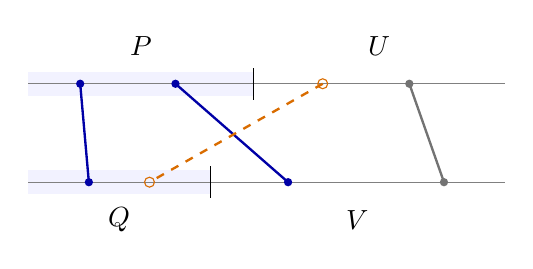
\begin{tikzpicture}[x=1.1cm,y=1.25cm,
  pair/.style={line width=0.85pt},
  removed/.style={pair,blue!65!black},
  kept/.style={pair,black!55},
  forbidden/.style={pair,dashed,orange!85!black}]
  \fill[blue!5] (0,0.88) rectangle (2.6,1.12);
  \fill[blue!5] (0,-0.12) rectangle (2.1,0.12);
  \draw[black!50] (0,1)--(5.5,1);
  \draw[black!50] (0,0)--(5.5,0);
  \draw (2.6,0.84)--(2.6,1.16);
  \draw (2.1,-0.16)--(2.1,0.16);
  \node at (1.3,1.38) {$P$};
  \node at (4.05,1.38) {$U$};
  \node at (1.05,-0.38) {$Q$};
  \node at (3.8,-0.38) {$V$};
  \draw[removed] (0.6,1)--(0.7,0);
  \draw[removed] (1.7,1)--(3.0,0);
  \draw[kept] (4.4,1)--(4.8,0);
  \draw[forbidden] (3.4,1)--(1.4,0);
  \foreach \x/\y in {0.6/1,0.7/0,1.7/1,3.0/0}
    \fill[blue!65!black] (\x,\y) circle (1.5pt);
  \foreach \x/\y in {4.4/1,4.8/0}
    \fill[black!55] (\x,\y) circle (1.5pt);
  \foreach \x/\y in {3.4/1,1.4/0}
    \draw[orange!85!black] (\x,\y) circle (1.8pt);
\end{tikzpicture}
\caption{A pair from $P$ to $V$ excludes a pair from $U$ to $Q$.
The dashed orange pair cannot belong to the order-preserving matching
containing the solid blue pair that crosses the prefix cuts.
All removed pairs can therefore be charged to source symbols in $P$.
The gray pair remains in the suffix alignment.}
\label{fig:overview-prefix-cut}
\end{figure}

When $\mu(P)=\mu(Q)$, the error term vanishes. This is precisely the
condition obtained when two comparable grid vertices have equal raw
offset. If $(i_2,j_2)$ has the same offset as $(i_1,j_1)$ and
$i_2\ge i_1$, strict growth of prefix mass implies $j_2\ge j_1$.
The fragments $X[i_1,i_2)$ and $Y[j_1,j_2)$ have equal mass.
Applying~\eqref{eq:overview-removal} to these removed prefixes shows that
the later vertex has no greater optimum remaining distance.

The inequality also justifies greedy match extension. Identical prefixes
have equal mass, so removing them cannot increase remaining distance.
Matching them for free proves the reverse comparison. A longest common
extension therefore changes neither the score, the raw offset, nor the
optimum remaining cost. The same structural statement supplies both
operations required by the frontier.

\subsection{Generated frontiers and feasible completions}

For integer costs, maintain an entry $R[c,d]$ for exact score $c$ and
mass offset $d$. An entry stores one generated vertex and its realizing
prefix alignment. Before comparing a candidate with the current record,
extend its common prefix. Retain the candidate with larger source index.
Equal offsets make the target indices ordered in the same direction, so
completion dominance applies to every such replacement.

Table~\ref{tab:overview-frontier-trace} follows selected transitions on
the counterexample. From the initial vertex, deleting $a$ and matching
$b$ reaches $(2,1)$ at score $1$. One branch substitutes the next $b$
by $c$. Another deletes that $b$, matches $c$, and inserts $a$.
The resulting score-$3$ records have different raw offsets and occupy
different entries. Their completions generate terminal candidates at
scores $4$ and $5$. The algorithm retains the cheaper completion while
remaining free to explore the other branch.

\begin{table}[t]
\centering
\small
\begin{tabular}{@{}ccclccc@{}}
\toprule
Record & From & Positive edit & Match run & Vertex & Score & Offset\\
\midrule
$S$ & none & none & none & $(0,0)$ & $0$ & $0$\\
$A$ & $S$ & delete $a$ & $b$ & $(2,1)$ & $1$ & $1$\\
$B$ & $A$ & delete $b$ & $c$ & $(4,2)$ & $2$ & $2$\\
$C$ & $A$ & $b\to c$ & none & $(3,2)$ & $3$ & $0$\\
$E$ & $B$ & insert $a$ & none & $(4,3)$ & $3$ & $1$\\
$T$ & $C$ & insert $a$ & $c$ & $(4,4)$ & $4$ & $-1$\\
$T'$ & $E$ & insert $c$ & none & $(4,4)$ & $5$ & $-1$\\
\bottomrule
\end{tabular}
\caption{Selected generated transitions for $X=\mathtt{abbc}$ and
$Y=\mathtt{bcac}$. Each row records one positive edit followed by maximal
match extension. Records $C,E$ have the same score and positional offset,
but different raw mass offsets. The table describes these transitions,
not the complete contents of each layer.}
\label{tab:overview-frontier-trace}
\end{table}

To prove completeness, fix the optimum value $D\le k$. A generated
label $(c,i,j)$ is \emph{feasible for completion} when
\[
 c+D(X[i:],Y[j:])\le D.
\]
Initialization is feasible. Match extension preserves feasibility, and
so does replacing a candidate by a farther record at the same $(c,d)$.
At a nonterminal extended vertex, an optimum remaining alignment starts
with a positive edit. The algorithm generates that edit, and its
candidate is still feasible. Any replacement at the destination entry
preserves feasibility again.

This argument follows a sequence of feasible representatives, rather
than a fixed optimum path through all its original vertices. A retained
vertex may expose different symbols from the discarded candidate.
Its suffix optimum is nevertheless no more expensive, which supplies
the next feasible transition. Strictly increasing integer scores bound
the sequence, and a feasible label at score $D$ must be terminal.
Every stored record has a realizing alignment, so no terminal score can
underestimate the distance. Lemma~\ref{lem:completion} formalizes this
completion invariant.

The invariant also identifies the information that a representative must
retain. Its exact score gives a realizing cost for the consumed prefixes;
its offset identifies the class in which replacement is safe; and its
two positions identify the remaining strings and the available next
edits. There is no need to retain all ways of reaching the same entry.
When the chosen representative changes, its realizing predecessor changes
with it. The suffix comparison then supplies the completion that the
discarded record would otherwise have preserved.

Incoming positive edits always originate in smaller score layers.
Consequently, all candidates for a layer have arrived before that layer
is processed. Its representatives are then final. This also explains
why the algorithm returns on processing a terminal entry, rather than
on generating a terminal candidate: edits of different costs can generate
terminal candidates out of score order.

\subsection{Global accounting and the numerical range}

The mass potential and integrality bound the entire state space:
$0\le c\le k$ and $-c\le d\le c$, with both coordinates integral.
The number of entries is
\[
 \sum_{c=0}^{k}(2c+1)=(k+1)^2.
\]
Each entry is processed once and generates at most three positive-edit
candidates. Each candidate takes one longest common extension query and
a constant number of arithmetic operations. Gap costs and prefix masses
are precomputed in linear time; substitution costs are queried when a
record is processed. Empty-entry scans, unsuccessful candidates, and
record replacements are all included in this count. Thus the bound
controls all generated work, not only the transitions followed in the
completeness argument.

An integer offset need not occur at any grid vertex. Such an entry simply
stays empty. The algorithm never searches for a vertex with a prescribed
mass or inverts the prefix-mass sequences: candidates already carry their
source and target positions, and their offset is obtained by two prefix
sum lookups. In particular, the implementation does not depend on the
number of missing mass values or on the total gap mass of the inputs.

An expensive symbol contributes a large jump in score or offset, but
does not create additional entries within the budget. To control retained
integer magnitudes, uniformly truncate the entire metric at $k+1$.
The truncated function remains a metric. Every alignment of cost at most
$k$ is unchanged, and no new such alignment can use a truncated edge,
since that edge alone would exceed the budget. Its gap costs define the
prefix masses used by the frontier. This operation preserves the gap
inequalities and differs from clipping coordinates while retaining the
old substitution costs.

After truncation, prefix masses are at most $n(k+1)$, and retained
integers require $O(\log(n+k+2))$ bits. The operation count assumes
constant-time metric queries and exact arithmetic; it does not measure
the representation cost of arbitrary oracle replies. Finally, each record
stores its generating edit and match length. Predecessors belong to final
smaller layers, so traceback remains valid when destination records are
replaced. The resulting alignment has at most $k$ positive edits, and
expanding its match runs costs $O(n)$.

\subsection{Rounding and separate score and gap granularities}

For a normalized real metric, every positive edit costs at least one.
An optimum alignment therefore contains at most $D$ positive edits.
Choose an integer $Q$ with $1/\eps\le Q<2/\eps$, and define
$w_Q(a,b)=\lceil Qw(a,b)\rceil$ for distinct symbols, with zero
diagonal. This definition includes the gap symbol. Upward rounding
preserves the metric because
$\lceil x+y\rceil\le\lceil x\rceil+\lceil y\rceil$.
Writing $D_Q$ for the rounded optimum gives
\[
 QD\le D_Q\le(Q+1)D.
\]
The first comparison holds for every alignment. The second applies
rounding to an original optimum, adding at most one per positive edit.
Thus $D_Q/Q$ is a $(1+\eps)$-approximation.

If $D\le k$, the rounded optimum is at most $(Q+1)k$. The integer
frontier at this budget has $O((Qk)^2)$ entries. A successful call
returns the exact rounded optimum and hence a valid approximation,
even when $D>k$. Failure certifies $D>k$. Capped rounded costs can be
queried by searching integer candidates with comparisons to $Qw(a,b)$;
this adds logarithmic overhead without requiring a real ceiling primitive.
The resulting bound is $\softO(n+(k/\eps)^2)$.

Score spacing and gap spacing need not coincide. If edit scores have
spacing $\eta$ and gap masses have spacing $\gamma$, there are
$O(1+k/\eta)$ score levels and $O(1+k/\gamma)$ offsets.
The same frontier consequently has a product bound. In particular, when
original gap costs are integers, rounded gaps are multiples of $Q$.
At rounded budget $O(Qk)$ there are $O(Qk)$ score levels but only
$O(k)$ offsets. This gives $\softO(n+k^2/\eps)$ approximation time.
A truncation cap chosen as a multiple of $Q$ preserves this gap lattice.
By trying original thresholds only while $Qk^2\le n^2$, then using
full dynamic programming if necessary, the same lattice gives
$\softO(n+\min\{D^2/\eps,n^2\})$ without a supplied threshold.
Section~\ref{sec:extensions} states the lattice guarantees and proves
the stopping rule for this stronger distance-sensitive bound.

\subsection{Removing the threshold and the scope of the method}

The bounded frontier also gives a distance-sensitive exact algorithm.
Handle equal strings first. Fix the metric cap $n+1$, preprocess once,
and try increasing dyadic budgets below $n$, followed by budget $n$.
The fixed cap preserves every tested bounded answer. If $D\le n$, the
first successful budget is at most $2D$, and the quadratic frontier costs
sum to $O(D^2)$. If all calls fail, then $D>n$; the original quadratic
dynamic program supplies the exact answer. Reusing preprocessing avoids
repeated input scans, and stopping at $n$ avoids searching an arbitrarily
large cost range. The total is $O(n+\min\{D^2,n^2\})$.

The real-cost approximation uses the same schedule on one capped rounded
metric. Success gives an optimum rounded alignment. If every call fails,
then $D_Q>n$, which implies $n=O(D/\eps)$; an original full-DP
fallback fits the claimed minimum bound. Very small accuracy parameters
are handled directly by full DP when $\eps<1/n$. In that case
$D\ge1$ for unequal strings, so $(D/\eps)^2>n^2$. This yields
$\softO(n+\min\{(D/\eps)^2,n^2\})$ without dependence on the metric's
numerical range.

Prefix removal remains valid for real metrics. Integrality enters only
when counting exact scores and offsets. A lower bound on each positive
edit does not separate the costs of competing alignments, so normalization
alone does not give a finite quadratic frontier. The structural argument
also uses only the two gap inequalities; the broader alignment-scoring
extension in Section~\ref{sec:extensions} exploits this fact. For the
metric results, these inequalities provide the lossless replacement
rule, and numerical granularity supplies the global state bound.

\section{Preliminaries}\label{sec:preliminaries}

\subsection{Strings, metric costs, and alignments}

Let $\Sigma$ be an alphabet and let $\gap\notin\Sigma$ be a gap symbol.
We write $\overline\Sigma=\Sigma\cup\{\gap\}$.
A string $Z\in\Sigma^*$ has positions $0,\ldots,|Z|-1$.
For $0\le i\le j\le|Z|$, the substring $Z[i,j)$ contains positions
$i,\ldots,j-1$, and $Z[i:]=Z[i,|Z|)$ is a suffix.
The empty string is denoted by $\emptyset$.
For the input strings, put $m=|X|$, $r=|Y|$, and $n=m+r$.
Both-empty inputs are handled in constant time. Resource bounds below
use $n\ge1$ and extend by an additive constant to that case.

The cost function $w:\overline\Sigma^2\to\mathbb R_{\ge0}$ is a metric:
it is symmetric, it is zero exactly on the diagonal, and it satisfies
the triangle inequality. Write
\[
 g(a)=w(a,\gap)\qquad(a\in\Sigma).
\]
Deleting or inserting $a$ costs $g(a)$, and substituting $a$ by $b$
costs $w(a,b)$. Substituting a symbol by itself is a match of cost zero.
The metric is \emph{normalized} when every nonzero value is at least one.
In particular, a metric with positive integer nonzero values is normalized.
The alphabet and cost function can vary with the input.

An edit sequence transforms one string into another by these operations.
The weighted edit distance $\WED_w(A,B)$ is its minimum total cost.
To compute the distance, we use the alignment grid for $A,B$.
Its vertices are $(i,j)$ with $0\le i\le|A|$ and $0\le j\le|B|$.
There are three types of directed edges, when the indicated symbols exist:
\[
\begin{array}{lll}
 (i,j)\longrightarrow(i+1,j)
   &\text{at cost }g(A[i])&\text{(deletion)},\\
 (i,j)\longrightarrow(i,j+1)
   &\text{at cost }g(B[j])&\text{(insertion)},\\
 (i,j)\longrightarrow(i+1,j+1)
   &\text{at cost }w(A[i],B[j])&\text{(diagonal)}.
\end{array}
\]
An alignment is a path from $(0,0)$ to $(|A|,|B|)$.
A diagonal edge between equal symbols is a match. Every other edge
has positive cost. Each edge increases at least one coordinate,
so the grid is acyclic and every alignment has at most $|A|+|B|$ edges.

For completeness, we establish the standard alignment formulation
used by the dynamic program~\cite{WF74}.

\begin{lemma}[Alignment formulation]\label{lem:alignment-formulation}
For metric costs, minimum alignment cost equals weighted edit distance.
\end{lemma}
\begin{proof}
First execute an alignment from left to right. Maintain a boundary
between the already produced target prefix and the unprocessed source
suffix. A deletion removes the first symbol of that suffix. An insertion
places the next target symbol at the boundary and advances the boundary.
A diagonal edge retains or substitutes the first source symbol and
advances the boundary. This gives an edit sequence with the same cost.

For the reverse direction, fix any finite edit sequence from $A$ to $B$.
Give each original character occurrence its own token. An insertion
creates a new token, a substitution changes the symbol of one token,
and a deletion destroys one token. Operations never change the relative
order of surviving tokens.
Pair each surviving original token with its final position in $B$.
These pairs form an order-preserving matching of source and target
positions.

The operations on a token form one history. If an original token
starts with symbol $a$ and survives with final symbol $b$, the triangle
inequality bounds the sum of its substitution costs from below by
$w(a,b)$. If an original token is eventually deleted, append $\gap$
to its symbol history. The substitutions and deletion then cost at
least $w(a,\gap)=g(a)$. If an inserted token survives with final symbol
$b$, prepend $\gap$ to its history. Its insertion and substitutions
cost at least $w(\gap,b)=g(b)$. An inserted token that is eventually
deleted has nonnegative total cost and contributes no final position.

Every operation belongs to exactly one token history. Summing these
bounds shows that the matching of surviving original tokens, together
with deletions of the unmatched source positions and insertions of the
unmatched target positions, costs no more than the edit sequence.
Order preservation lets us realize these operations as an alignment.
Taking minima in both directions proves the equality.
\end{proof}

For a fixed metric, write $D(A,B)=\WED_w(A,B)$.
The grid has finitely many paths, so an optimal alignment exists.
An optimal path has optimal subpaths: replacing a subpath by a cheaper
path with the same endpoints would improve the full path.
In particular, the part of an optimal alignment following a vertex
$(i,j)$ is optimal for the suffixes $A[i:]$ and $B[j:]$.

\subsection{Full dynamic programming and its output}

We will use full dynamic programming only when its quadratic cost fits
the claimed bound. Here we give its recurrence and reconstruction
explicitly.
Let $F[i,j]$ be the optimum alignment cost for $X[0,i),Y[0,j)$.
Initialize
\begin{equation}\label{eq:dp-boundaries}
 F[0,0]=0,\qquad
 F[i,0]=\sum_{p=0}^{i-1}g(X[p]),\qquad
 F[0,j]=\sum_{q=0}^{j-1}g(Y[q]).
\end{equation}
For $i,j>0$, set
\begin{equation}\label{eq:full-dp}
 F[i,j]=\min\left\{
 \begin{aligned}
  &F[i-1,j]+g(X[i-1]),\\
  &F[i,j-1]+g(Y[j-1]),\\
  &F[i-1,j-1]+w(X[i-1],Y[j-1]).
 \end{aligned}\right\}.
\end{equation}
The algorithm fills the array in row-major order and records one
minimizing incoming edge for every nonroot entry. Ties can be resolved
in a fixed order.

The boundary entries have only deletion or only insertion paths.
For an interior entry, the last edge of every alignment is one of the
three edges in~\eqref{eq:full-dp}. Removing that edge leaves an alignment
for its predecessor vertex. Conversely, an optimum predecessor path
followed by the indicated edge is a valid path to $(i,j)$.
Induction on $i+j$ therefore proves the recurrence and gives
$F[m,r]=D(X,Y)$.

To recover an alignment, start at $(m,r)$ and follow the recorded edges
back to $(0,0)$. A deletion produces the column $(X[i-1],\gap)$,
an insertion produces $(\gap,Y[j-1])$, and a diagonal edge produces
$(X[i-1],Y[j-1])$. Reverse the collected columns to obtain the alignment
in its forward order. Each step decreases at least one coordinate,
so reconstruction takes $O(n+1)$ time. The recorded predecessor choices
give the realizing path for the value computed at each entry, and hence
the reconstructed alignment is optimal.

Cache the $n$ gap costs before filling the array. There is one
substitution-cost query and a constant number of arithmetic operations
at each interior entry. The number of entries is
$(m+1)(r+1)=1+n+mr$. Thus full computation and predecessor storage take
$O(1+n+mr)$ time and space, including reconstruction.
This statement uses the exact cost-arithmetic model specified below.
In a fallback call, the recurrence uses the original metric, even when
earlier bounded calls used a truncated one.

\subsection{Order-preserving matchings and gap masses}

An alignment can also be specified by the source and target positions
paired by its diagonal edges. These pairs form an order-preserving
matching $M$: each position occurs in at most one pair, and
$(i,j),(i',j')\in M$ with $i<i'$ satisfy $j<j'$.
Conversely, an order-preserving matching gives an alignment by processing
its pairs in order and deleting or inserting the intervening unmatched
positions. Different orders of intervening deletions and insertions
have the same cost.

For a string $Z$, define its gap mass and prefix masses by
\[
 \mu(Z)=\sum_{p=0}^{|Z|-1}g(Z[p]),\qquad
 \mu_Z(i)=\mu(Z[0,i)).
\]
For the input grid, define the mass offset
\[
 \delta(i,j)=\mu_X(i)-\mu_Y(j).
\]
Positive gap costs make each prefix-mass sequence strictly increasing.
The triangle inequalities involving $\gap$ give
\begin{equation}\label{eq:gap-inequalities}
 |g(a)-g(b)|\le w(a,b)\le g(a)+g(b).
\end{equation}
The upper inequality uses the path through $\gap$.
The lower one follows by applying the triangle inequality to
$w(a,\gap)$ and $w(b,\gap)$ separately.

Relative to deleting $a$ and inserting $b$, pairing them saves
\begin{equation}\label{eq:savings}
 s(a,b)=g(a)+g(b)-w(a,b),\qquad
 0\le s(a,b)\le2\min\{g(a),g(b)\}.
\end{equation}
The lower bound follows from the upper gap inequality.
For the upper bound, subtract the lower gap inequality from
$g(a)+g(b)$.
Consequently, the alignment specified by a matching $M$ on strings $A,B$
has cost
\begin{equation}\label{eq:matching-cost}
 \mu(A)+\mu(B)-\sum_{(i,j)\in M}s(A[i],B[j]).
\end{equation}
Indeed, deleting all source positions and inserting all target positions
gives the baseline $\mu(A)+\mu(B)$. Each matched pair replaces the
corresponding deletion and insertion by one diagonal edge.
The matching and savings formulation is standard; it also appears
in the metric approximation framework of~\cite[Section~4]{DKK26}.

The prefix-mass potential below is explicit in
Das, Kipouridis, and Kociumaka~\cite[Lemma~3.2]{DKK26}.
We prove it here for the raw masses used throughout the algorithm.

\begin{lemma}[Mass potential]\label{lem:potential}
An alignment subpath from $(i,j)$ to $(i',j')$ with cost $c$ satisfies
\[
 |\delta(i',j')-\delta(i,j)|\le c.
\]
In particular, a path from $(0,0)$ of cost $c$ reaches only vertices
with $|\delta|\le c$.
\end{lemma}
\begin{proof}
A deletion of $a$ changes the offset by $g(a)$, and an insertion of
$b$ changes it by $-g(b)$. In either case the absolute change equals
the edge cost. A diagonal edge pairing $a,b$ changes the offset by
$g(a)-g(b)$, whose absolute value is at most $w(a,b)$ by
\eqref{eq:gap-inequalities}. The absolute value of the sum of the offset
changes is at most the sum of their absolute values, which is at most
the path cost.
The final assertion uses $\delta(0,0)=0$.
\end{proof}

Masses always use the gap costs of the metric currently scoring the
alignment. In particular, after truncating or rounding the metric,
the algorithm recomputes masses from that metric. Independently clipping
the masses while retaining the old edit costs would give different
coordinates and is not the operation used in our exact argument.

\subsection{Computation and output conventions}\label{sec:model}

We use an exact oracle arithmetic model. A query to $w$ returns the
exact cost of the specified symbol pair. Queries, addition, subtraction,
multiplication, division, and comparison take constant time.
These assumptions count operations and queries rather than the bit cost
of reading or manipulating an arbitrary cost representation.
The metric axioms are an input promise; no algorithm reads or validates
a complete $|\overline\Sigma|^2$ table.

The string representation is the standard integer-alphabet model.
Input symbols have integer codes bounded by $n^{c_{\rm alph}}$ for a
fixed constant $c_{\rm alph}$, stored in $O(\log(n+2))$-bit words.
Word access and the usual integer word operations take constant time.
The alphabet may grow with the input. Its string representation is
separate from the exact registers holding metric values.
Section~\ref{sec:lce} gives a deterministic implementation of the
following LCE interface and proves its bounds in
Lemma~\ref{lem:lce-index}.

After $O(n)$ preprocessing time and space, a query at $(i,j)$ returns
the longest common-prefix length
\[
 \ell=\lce(X[i:],Y[j:])
\]
in $O(1)$ time. The answer is bounded by both remaining suffix lengths.
If either suffix is empty, the answer is zero.
Write $\Ext(i,j)=(i+\ell,j+\ell)$.
The index depends only on the input strings, so it can be reused after
changing the scoring metric or the budget.
For other string representations, an LCE implementation with
preprocessing time $P(n)$ and query time $T_{\rm LCE}(n)$ adds its
preprocessing cost and multiplies the frontier's LCE-query work by
$T_{\rm LCE}(n)$.

For bounded integer computation, whole-metric truncation ensures that
the integers retained in the frontier and mass arrays have
$O(\log(n+k+2))$ bits. The approximation likewise stores only bounded
integer indices and rounded values; its scale and register bounds are
specified in Section~\ref{sec:approximation}. Its real-valued metric
replies remain exact oracle registers. The algorithms do not convert
unrestricted real values to integers or extract digits from those values.
An original-metric full-DP fallback can store scores of arbitrarily large
numerical magnitude. Its stated operation bound uses the same exact
arithmetic assumption.

An exact bounded call returns the distance and an optimal alignment
when the distance is at most its threshold; otherwise it reports that
the threshold is exceeded. We represent an alignment by the initial
match-run length followed by blocks consisting of one positive edit and
the length of its following match run. An edit descriptor records its
type and the source and target boundaries at which it is applied.
This representation has $O(n+1)$ size, and expanding it into alignment
columns takes $O(n+1)$ time.

A bounded approximation call returns an estimate $A$ and an alignment
of original cost at most $A$, with $D\le A\le(1+\eps)D$, or reports
$D>k$. It must return an approximation whenever $D\le k$.
A successful call can also occur when $D>k$, but its estimate and
alignment must still satisfy the same inequalities.
In bounded approximation bounds, $\softO$ hides factors polynomial in
$\log(n+k/\eps+2)$. In the distance-sensitive approximation it hides
factors polynomial in $\log(n+2)$. Hidden constants are independent
of the input metric and of $\eps$. Comparisons with previous algorithms
use their stated logarithmic conventions.

\subsection{Longest common extension preprocessing}\label{sec:lce}

This subsection implements the longest common extension operation used by
the frontier. All operations in this subsection concern character codes,
positions, and lengths. They do not access the metric oracle. We use
word-sized integer addition, subtraction, comparison, multiplication,
bit operations, shifts, and array access. The word length is
$\Theta(\log(n+2))$, with a sufficiently large constant to hold the
input character codes. Integer logarithms and block indices are
precomputed below; no operation converts a metric value to an integer.
This construction supplies the string primitive used by the weighted
frontier in Section~\ref{sec:integer}.

The construction has three parts. We first order the suffixes of a
combined text. We then compute the longest common prefixes of adjacent
suffixes. Finally, we index range minima of those prefix lengths.
The familiar constructions underlying these parts are due to
K\"arkk\"ainen and Sanders~\cite{KS03},
Kasai et al.~\cite{KLAAP01}, and Bender and
Farach-Colton~\cite{BF00}, respectively. We give the algorithms and
their proofs here, including the boundary conventions needed by our
queries.

\subsubsection{The text and integer sorting}\label{sec:lce-text}

Let $m=|X|$, $r=|Y|$, and $n=m+r$. Input character codes belong to
$[0,n^{c_\alpha}]$ for a fixed constant $c_\alpha$. Replace the
distinct occurring codes by ranks $1,\ldots,d$ in increasing order,
then add two to every rank. Ordinary character codes are therefore at
least three. This replacement preserves equality and order.
Introduce two distinct sentinels $\#_X,\#_Y$ with codes $1,2$ and form
\[
 T=X\#_X Y\#_Y,\qquad N=|T|=n+2.
\]
Every actual text code is positive. We use code $0$ only as virtual
padding beyond the text. The sentinels occur exactly once each and do
not belong to the original alphabet.

Here is the sorting implementation used for the initial replacement
and for tuples later in the construction. For $q$ records whose keys
belong to $[0,U]$, counting sort takes $O(q+U+1)$ time and words.
Initialize one counter per key, count the records, and compute the
starting offset of each key from the prefix sums of the counters.
Scan the records in their original order. Place a record at the next
unused offset for its key and increment that offset. Records with an
equal key keep their relative order. This proves both the ordering and
the stability of the pass.

To sort $n$ polynomially bounded character codes, choose a power of
two $B$ with $N\le B<2N$. Repeated doubling finds $B$ and its exponent
in $O(\log N)$ time. Represent a character code in base $B$. A
constant number of digits suffices because $c_\alpha$ is fixed.
Sort successively by the least significant digit, the next digit,
and so on. Each digit lies in $[0,B)$, so each stable counting-sort
pass takes $O(N)$ time. Induction on the passes shows that the records
are sorted by the processed low-order digits; after the last pass
they are sorted by their entire codes. A scan assigns an equal rank
to equal codes and increasing ranks to increasing codes. The total
time and space are $O(N)$.

Tuples of a fixed number of integer components in $[0,O(q)]$ can be
sorted in $O(q)$ time by the same method: apply stable counting sort
to the last component first and the first component last. We will
use only pairs and triples. These sorting calls have linear-sized
key ranges and a constant number of passes.

\subsubsection{Linear-time suffix ordering}\label{sec:lce-suffix}

We describe a recursive algorithm for a positive-integer string
$S[0,L)$ with alphabet contained in $[1,O(L)]$. Its output orders
all suffixes $S[p,L)$ for $p\in[0,L]$, including the empty suffix
at $p=L$. Set $S[p]=0$ for every $p\ge L$ when constructing a
tuple or making a comparison. The empty suffix is smaller than
every nonempty suffix. This agrees with comparison of the padded
strings, because actual character codes are positive.

If $L\le2$, compare the at most three suffixes directly. Each
comparison reads at most two characters. Assume below that $L\ge3$.
Partition the suffix positions into residue classes
\[
 B_a=\{p\in[0,L]:p\equiv a\pmod3\},\qquad a\in\{0,1,2\},
 \qquad C=B_1\cup B_2.
\]
In particular, $L$ belongs to $C$ if $L\bmod3\ne0$. This convention
supplies the empty suffix as a sample exactly when it is needed in
that residue class. There is no unmentioned dummy suffix.
The number of samples is
\[
 |C|=L-\lfloor L/3\rfloor=\lceil2L/3\rceil.
\]

\paragraph{Order the sample suffixes.}
For each $p\in C$, form the triple
$\tau_p=(S[p],S[p+1],S[p+2])$. Sort the triples and assign their
distinct values names $1,2,\ldots,d$ in increasing lexicographic
order. Thus equal triples have equal names and the order of names
is the order of triples. Write $\nu_p$ for the name of $\tau_p$.
Concatenate the two sequences of names, each listed in increasing
position order:
\[
 R=(\nu_p:p\in B_1\text{ in increasing order})\,
   (\nu_p:p\in B_2\text{ in increasing order}).
\]
Store the bijection $\phi$ from positions of $R$ to sample positions
of $S$. Recursively order all suffixes of $R$, discard its empty
suffix, and apply $\phi$ to the remaining positions. The result is
the order of the sample suffixes of $S$.

The following boundary argument justifies this reduction for every
value of $L\bmod3$. In either residue sequence, only its final
triple contains a zero. The final triples of the two sequences are
distinct: they contain different numbers of trailing zeros. The
possibilities are
\[
\begin{array}{c|cc}
 L\bmod3 & \text{last triple in }B_1 &
                 \text{last triple in }B_2\\\hline
 0 & (S[L-2],S[L-1],0) & (S[L-1],0,0)\\
 1 & (0,0,0) & (S[L-2],S[L-1],0)\\
 2 & (S[L-1],0,0) & (0,0,0).
\end{array}
\]
Actual character codes are positive, so both final triples are
unique among all sampled triples. A sampled suffix beginning at
$p$ consists of successive triples at $p,p+3,\ldots$, ending in
the final triple of its residue sequence. Comparing these triple
sequences gives the order of the original suffixes. Zero padding
makes a shorter suffix smaller at its first missing character.

Consider two distinct sample positions $p,q$. Their triple
sequences differ before either comparison passes its final triple.
Indeed, if a final triple were equal to a triple in the other
sequence, uniqueness would force both triples to have the same
starting position. Since the comparisons advanced by the same
number of triples, this would force $p=q$. Names preserve the
order at the first different triple. Consequently, the extra
$B_2$ names following the $B_1$ sequence in $R$ cannot change a
comparison. This proves the order-preserving correspondence of
suffixes used by the recursive call.

Assign increasing positive ranks to the ordered nonempty sample
suffixes, beginning with rank $1$. Define $\rho_L=0$ for the empty
suffix, whether or not it was sampled, and $\rho_p=0$ for every
$p>L$. For sampled positions $p<L$, let $\rho_p$ be their assigned
rank. These values encode exactly the relative order of the sample
suffixes and the empty suffix. Ranks at nonsample positions below
$L$ are not needed or defined.

\paragraph{Order the remaining suffixes.}
For $p\in B_0$, use the key
\[
 (S[p],\rho_{p+1}).
\]
If $p<L$, position $p+1$ is sampled unless it is the empty
suffix. If $p=L$, both components are zero. The key therefore
consists of the first character and the rank of the remaining
suffix. Lexicographic ordering of these keys orders the suffixes
in $B_0$ exactly. Two counting-sort passes give this order in
$O(L)$ time.

\paragraph{Merge the two orders.}
Merge the ordered lists for $C$ and $B_0$. To compare a sample
suffix at $p$ with a nonsample suffix at $q$, use
\[
\begin{array}{ll}
 p\bmod3=1:
   &(S[p],\rho_{p+1})\text{ versus }(S[q],\rho_{q+1}),\\[0.3em]
 p\bmod3=2:
   &(S[p],S[p+1],\rho_{p+2})\text{ versus }
     (S[q],S[q+1],\rho_{q+2}).
\end{array}
\]
In the first case, both rank positions have residues $2$ or $1$.
In the second case, they have residues $1$ or $2$. Hence every
referenced rank is defined, including ranks of empty or padded
suffixes. After comparing one or two initial characters, the
rank comparison gives the order of the remaining suffixes.
Each comparison takes constant time. The usual merge, which
outputs the smaller head and advances its list, uses at most
$L$ comparisons and produces all $L+1$ suffixes in order.

All arrays, sorting passes, and comparisons outside the recursive
call use $O(L)$ time and words. The recursive string has length
$\lceil2L/3\rceil$ and alphabet size at most that length. Therefore
\[
 F(L)\le F(\lceil2L/3\rceil)+O(L),\qquad F(L)=O(1)\text{ for }L\le2.
\]
For $L\ge8$, the next length is at most $3L/4$; the remaining
constant-sized case takes constant work. The sum of lengths over
the recursion is consequently $O(L)$. This proves an $O(L)$
time bound. The same geometric sum bounds simultaneously retained
arrays by $O(L)$ words. Applying the algorithm to $T$ gives its
suffix array $\mathrm{SA}[0,N]$ and inverse array $\mathrm{rank}[0,N]$.
In particular, $\mathrm{SA}[0]=N$.

\subsubsection{Adjacent longest common prefixes}\label{sec:lce-lcp}

For $t\in[1,N]$, let
\[
 H[t]=\operatorname{LCP}
    \bigl(T[\mathrm{SA}[t-1],N),T[\mathrm{SA}[t],N)\bigr),
 \qquad H[0]=0.
\]
We compute $H$ in order of text positions, rather than suffix
array positions. Initialize $h=0$. For $p=0,1,\ldots,N-1$, let
$t=\mathrm{rank}[p]$ and $q=\mathrm{SA}[t-1]$. Since $p<N$,
the suffix is nonempty and $t\ge1$. Starting with the current $h$,
increment $h$ while both $p+h<N$ and $q+h<N$ and
$T[p+h]=T[q+h]$. Set $H[t]=h$, then replace $h$ by
$\max\{h-1,0\}$. The test handles $q=N$, the empty predecessor,
without reading an out-of-range character.

To prove correctness, we first record a property of lexicographic
order. If two strings share a prefix of length $a$, every string
between them in lexicographic order shares that prefix. A string
that first differs before position $a$ is smaller than both or
larger than both, according to the differing character. A string
that ends before position $a$ is smaller than both. These cases
prove the property.

Suppose the exact predecessor common-prefix length at position
$p$ is $h>0$, and its predecessor begins at $q$. The first
characters agree. Removing these first characters preserves the
strict order, so
\[
 T[q+1,N)<T[p+1,N).
\]
These two suffixes share a prefix of length $h-1$. The immediate
predecessor of $T[p+1,N)$ is lexicographically between them, or
equals $T[q+1,N)$. The interval property implies that this
predecessor shares a prefix of length at least $h-1$. If $h=0$,
zero is a valid lower bound for the next iteration. This proves
inductively that the initial value of $h$ in each iteration is a
valid lower bound. The character comparisons extend it to the
exact value, which proves the computation of $H$.

Every successful comparison increments $h$, and each of the $N$
iterations decreases $h$ by at most one. The variable remains
between $0$ and $N$. Thus there are at most $2N$ increments over
the entire computation. There is at most one unsuccessful
character comparison per iteration. All other operations are
constant per iteration, so the time and extra space are $O(N)$.

If $u<v$ are suffix-array ranks, then
\begin{equation}\label{eq:lce-rmq-identity}
 \operatorname{LCP}
   \bigl(T[\mathrm{SA}[u],N),T[\mathrm{SA}[v],N)\bigr)
   =\min_{t\in[u+1,v]} H[t].
\end{equation}
Let the minimum on the right be $a$. Successive adjacent suffixes
share their first $a$ characters, so the two endpoint suffixes
also share them. Conversely, if the endpoints share $b$ characters,
the interval property implies that every suffix between them
shares those characters. Every adjacent pair has common-prefix
length at least $b$, so $a\ge b$. These two inequalities prove
the identity.

\subsubsection{A linear-space constant-time range-minimum index}
\label{sec:lce-rmq}

We give a range-minimum index for a word-sized integer array
$A[0,M)$ with $M\ge1$, with a query returning the leftmost minimum position
in a nonempty interval $[i,j]$. We use it with $A=H$ and
$M=N+1$. The construction reduces arbitrary range minima to
range minima in a sequence whose adjacent values differ by one.

\paragraph{Cartesian tree.}
Associate the distinct ordered key $(A[t],t)$ with each position
$t$. Construct a binary tree whose inorder sequence is
$0,1,\ldots,M-1$ and whose keys increase from parent to child.
Here is a linear-time construction. Maintain a stack containing
the rightmost root-to-leaf path of the tree on the processed
prefix. On inserting position $t$, set $\mathit{last}$ to null
and pop stack entries while their keys exceed the key of $t$,
assigning each popped entry to $\mathit{last}$. If the stack is
nonempty, make $t$ its top entry's right child. Otherwise make
$t$ the root. Make $\mathit{last}$ the left child of $t$ when
it is nonnull. Set the corresponding parent pointers and push
$t$. All newly allocated child pointers are initially null.

The popped entries form the final part of the old rightmost
path. Their highest entry, which is the last one popped, roots
the subtree placed to the left of $t$. The unpopped top, if
present, has a smaller key and becomes $t$'s parent. All keys
in the moved subtree exceed the new key by the old heap order.
The new tree retains inorder positions and heap order, and its
rightmost path is exactly the new stack. This proves the
invariant by induction. Every position is pushed once and
popped at most once, so the time and space are $O(M)$.

For positions $i\le j$, their lowest common ancestor in this
tree is the leftmost minimum position in $[i,j]$. To see this,
let the ancestor be $v$. If one position is an ancestor of the
other, then $v$ is an endpoint. Otherwise the two positions
belong to different child subtrees of $v$, so inorder traversal
places $v$ between $i$ and $j$. The subtree of $v$ contains
every position in this interval. Heap order makes $v$'s key
smaller than the keys of the other positions there. The
second key component resolves equal array values to the
leftmost position, proving the claim.

\paragraph{Euler walk.}
Traverse each tree edge twice by a depth-first traversal. Record
the root initially, and record the current vertex after every
edge traversal. This produces a vertex sequence $V$ of length
$P=2M-1$. Record its depth sequence $E$ and the first occurrence
$f[v]$ of each vertex. Consecutive entries of $E$ differ by
$+1$ or $-1$.

The lowest common ancestor of vertices $i,j$ is the vertex of
minimum depth in the interval
$[\min\{f[i],f[j]\},\max\{f[i],f[j]\}]$. Throughout this
interval the walk stays in the subtree of their lowest common
ancestor and visits that ancestor. It cannot leave the subtree
before both first visits, because depth-first traversal completes
a subtree before leaving it. If one vertex is an ancestor of
the other, that ancestor is already an endpoint occurrence.
Otherwise the walk passes through it between the two child
subtrees. It is the only vertex at its depth inside this
subtree. This proves the minimum-depth characterization.

\paragraph{Small blocks.}
Precompute integer logarithms
$\lambda[t]=\lfloor\log_2t\rfloor$ for $1\le t\le P$ by
$\lambda[1]=0$ and
$\lambda[t]=1+\lambda[\lfloor t/2\rfloor]$ for $t\ge2$.
The division by two is an integer shift. Choose
\[
 b=\max\{1,\lfloor\lambda[P]/4\rfloor\}.
\]
Partition the Euler sequence into consecutive blocks of length
$b$, with a possibly shorter final block. In a scan, store for
each sequence position its block number and its position within
the block. These stored values avoid division at query time.

A full block is determined, up to an additive depth constant,
by its $b-1$ signs. Encode $+1$ by bit $1$ and $-1$ by bit $0$.
Pad a shorter final block with artificial $+1$ steps to length
$b$; no query uses a padded position. For every one of the
$2^{b-1}$ sign patterns, compute relative depths starting at
zero. For each pair $0\le a\le z<b$, store the leftmost
minimum position among these relative depths on $[a,z]$.
For each fixed $a$, a scan over $z$ maintains this minimum,
so one pattern costs $O(b^2)$ time and space. The total is
\[
 O(2^{b-1}b^2)=O(P^{1/4}\log^2(P+2))=O(P).
\]
For bounded $P$ the table has constant size; the displayed
asymptotic bound applies as $P$ grows. Encode all actual blocks
in another $O(P)$-time scan. A query wholly inside one block
now reads one table entry and adds the block's starting
position. The additive depth constant does not affect the
minimum position.

\paragraph{Complete blocks.}
Let $K=\lceil P/b\rceil$ be the number of blocks. Store a
minimum-depth sequence position $B[a]$ for each block $a$,
using only its valid positions. The block scan computes these
positions in $O(P)$ time. Compare candidate positions by the
pair $(E[t],t)$.

Construct a table $J[h,a]$ of minimum positions over the
$2^h$ consecutive blocks starting at $a$, for every interval
that fits. Set $J[0,a]=B[a]$. For $h>0$, compare
$J[h-1,a]$ and $J[h-1,a+2^{h-1}]$ and store the better
position. This recurrence computes each entry in constant
time. Its number of entries is
\[
 O(K\log(K+2))=O(P).
\]
Indeed, when $P$ is sufficiently large,
$b\ge (\log_2 P)/8$ and $K\le P/b+1$; substitute these
inequalities into the left side. The finitely many smaller
values are covered by a constant factor. Powers of two are
generated by successive shifts. No sorting or logarithm
oracle is used here.

To query a nonempty interval of full blocks $[a,z]$, let
$h=\lambda[z-a+1]$. Its minimum is the better of
\[
 J[h,a]\quad\text{and}\quad J[h,z-2^h+1].
\]
Both tabulated intervals lie inside the requested interval,
and their union covers it because
$2^h\le z-a+1<2^{h+1}$. Their possible overlap is harmless
for a minimum query. This proves the constant-time query.

\paragraph{General queries.}
A range of Euler positions lies in one block, or consists
of a suffix of its first block, zero or more whole blocks,
and a prefix of its final block. In the first case use the
pattern table. In the second case use two pattern-table
queries and, if present, one complete-block query. Compare
the at most three candidates and return the best. Each
query takes constant time. The resulting position of the
minimum depth gives the lowest common ancestor and hence
the original range-minimum position in $A$.

The Cartesian tree, Euler walk, logarithm array, block
patterns, pattern table, and complete-block table all take
$O(M)$ preprocessing time and words. All integers and bit
patterns use $O(\log(M+2))$ bits. This establishes the
claimed index without a range-minimum or lowest-common-
ancestor subroutine.

\Needspace{14\baselineskip}
\subsubsection{The longest common extension contract}
\label{sec:lce-contract}

\begin{lemma}[Longest common extension index]\label{lem:lce-index}
Let $X,Y$ have total length $n$ and character codes in
$[0,n^{c_\alpha}]$ for a fixed constant $c_\alpha$. A
deterministic word-RAM algorithm preprocesses the strings
in $O(n+1)$ time and space and answers each query
\[
 \lce(i,j)=\max\{\ell\in\mathbb Z_{\ge0}:
       X[i,i+\ell)=Y[j,j+\ell),\quad
       i+\ell\le|X|,\ j+\ell\le|Y|\}
\]
in $O(1)$ time, for $0\le i\le|X|$ and $0\le j\le|Y|$.
The answer is zero when either queried suffix is empty.
All stored integers use $O(\log(n+2))$ bits, and no metric
query or operation on a metric value is required.
\end{lemma}

\begin{proof}
Construct $T$, its suffix order, the adjacent-prefix array
$H$, and the range-minimum index as described above. Each
step takes $O(N)=O(n+1)$ time and space. For a query with
$i=|X|$ or $j=|Y|$, return zero. Otherwise compare the
suffixes of $T$ at positions $i$ and $|X|+1+j$. Their
positions are distinct, so their suffix-array ranks are
distinct. If these ranks in increasing order are $u<v$,
query the minimum of $H$ on $[u+1,v]$.
Equation~\eqref{eq:lce-rmq-identity} proves that this is
their longest common prefix in $T$. When either original
suffix reaches its end, its next character is its own
sentinel. That sentinel differs from every ordinary
character and from the other sentinel. The common prefix
therefore stops at or before this boundary. Its length is
exactly the requested finite-string answer. The rank
lookups and range-minimum query take constant time.
\end{proof}

The same index also supports queries between two positions
of one input string: cap the answer by the two remaining
input lengths, and return that remaining length directly
when the text positions coincide. The frontier requires
only the cross-string contract in
Lemma~\ref{lem:lce-index}. The virtual padding in suffix
ordering is an internal construction convention. The
index never treats padding or sentinels as an input match.

\section{Exact computation for integer metrics}\label{sec:integer}

We develop a bounded frontier subroutine, prove its correctness, and then
give the two interfaces in Theorem~\ref{thm:integer}. The bounded interface
uses a cap determined by its threshold. The distance-sensitive interface
uses one fixed capped metric and one preprocessing pass for every budget.

\subsection{Prefix-mass dominance}\label{sec:dominance}

The mass potential bounds how far an alignment can deviate in mass
coordinates. The next inequality concerns a different operation: removing
the consumed prefixes and comparing optimum remaining costs. It is the
structural basis of representative replacement.

\begin{lemma}[Prefix removal]\label{lem:removal}
For all strings $P,Q,U,V$,
\begin{equation}\label{eq:removal}
 D(U,V)\le D(PU,QV)+|\mu(P)-\mu(Q)|.
\end{equation}
\end{lemma}
\begin{proof}
Take an optimal matching between $PU$ and $QV$, and remove all pairs
that touch $P$ or $Q$. The remaining pairs form a matching between
$U$ and $V$.

If a pair connects $P$ to $V$, no pair can connect $U$ to $Q$,
because the two pairs would cross. Every removed pair then has its
source in $P$. Its total saving is at most $2\mu(P)$,
by~\eqref{eq:savings}. If no pair connects $P$ to $V$, every removed
pair has its target in $Q$, and its total saving is at most $2\mu(Q)$.
In either case the lost saving is at most
$2\max\{\mu(P),\mu(Q)\}$.

The baseline in~\eqref{eq:matching-cost} decreases by
$\mu(P)+\mu(Q)$. The cost of the remaining matching is therefore at most
\[
 D(PU,QV)-\mu(P)-\mu(Q)+2\max\{\mu(P),\mu(Q)\}
 =D(PU,QV)+|\mu(P)-\mu(Q)|.
\]
Taking the optimum for $U,V$ proves the claim.
\end{proof}

\begin{corollary}[Completion dominance]\label{cor:dominance}
Suppose $i_2\ge i_1$ and $j_2\ge j_1$. Then
\[
 D(X[i_2:],Y[j_2:])\le D(X[i_1:],Y[j_1:])
       +|\delta(i_2,j_2)-\delta(i_1,j_1)|.
\]
If the two offsets are equal, the later vertex has no greater remaining
distance. Moreover, two vertices with equal offsets are coordinatewise
ordered by their source indices.
\end{corollary}
\begin{proof}
Apply Lemma~\ref{lem:removal} with
$P=X[i_1,i_2)$ and $Q=Y[j_1,j_2)$. Their mass difference is the
difference of the offsets. If the offsets are equal and $i_2\ge i_1$,
then $\mu_Y(j_2)-\mu_Y(j_1)=\mu_X(i_2)-\mu_X(i_1)\ge0$.
Strictly increasing prefix masses imply $j_2\ge j_1$.
\end{proof}

\begin{corollary}[Common-prefix cancellation]\label{cor:cancellation}
For all strings $P,U,V$, $D(PU,PV)=D(U,V)$.
\end{corollary}
\begin{proof}
Lemma~\ref{lem:removal} gives $D(U,V)\le D(PU,PV)$. Matching $P$ for
free and following an optimal alignment of $U,V$ gives the reverse
inequality.
\end{proof}

\begin{lemma}[Safe match extension]\label{lem:extension}
If $(i',j')=\Ext(i,j)$, then
$\delta(i',j')=\delta(i,j)$ and
$D(X[i':],Y[j':])=D(X[i:],Y[j:])$.
At an extended nonterminal vertex, every remaining alignment starts with
a positive-cost edit.
\end{lemma}
\begin{proof}
The matched source and target prefixes are identical and have equal
gap mass. Thus offset is preserved, and
Corollary~\ref{cor:cancellation} gives the distance equality. At a
nonterminal extended vertex, either one suffix is empty or the next
symbols are distinct. None of its outgoing edges then has cost zero.
\end{proof}

\paragraph{Scope of the inequality.}
Lemma~\ref{lem:removal} does not require integer values. It uses only
positive gap costs and~\eqref{eq:gap-inequalities}. Integrality enters
later, when bounding the number of frontier entries. The matching
restriction is made at prefixes, where order preservation gives the
one-sided savings charge.

\subsection{The bounded cost--mass frontier}\label{sec:frontier}

\paragraph{Uniform metric truncation.}

The following elementary operation controls stored integer magnitudes.
It must be applied to the entire metric, including substitutions.

\begin{lemma}[Uniform truncation]\label{lem:truncation}
For every $C>0$, the function $w_C(a,b)=\min\{w(a,b),C\}$ is a
metric. If $C>k$, then $w_C$ and $w$ have the same bounded answer at
threshold $k$, and the same alignments of cost at most $k$.
\end{lemma}
\begin{proof}
Symmetry, zero diagonal, and positive off-diagonal values are preserved.
For the triangle inequality, use
\[
 \min\{w(a,c),C\}\le\min\{w(a,b)+w(b,c),C\}
 \le\min\{w(a,b),C\}+\min\{w(b,c),C\}.
\]
An alignment of truncated cost at most $k$ cannot contain an edge whose
truncated cost is $C$. All its costs therefore equal their original
values. Conversely, every original alignment of cost at most $k$ is
unchanged. The bounded optima coincide, including the failure case.
\end{proof}

For the subroutine below, fix any positive integer metric $v$ and an integer
budget $K\ge0$. Preprocess the LCE structure and the gap and prefix masses of
$v$. In this subsection and its proof, $g,\mu$, and $\delta$ use $v$,
and $D_v(A,B)$ denotes its alignment distance. The subroutine does not
change $v$ when it is called with a new budget.

\paragraph{Frontier records.}

For every integer $0\le c\le K$ and $-c\le d\le c$, allocate an
entry $R[c,d]$. A nonempty record has five fields
\[
 (i,j,p,e,\ell).
\]
Its vertex is $(i,j)$, its prefix alignment has exact cost $c$, and
$\delta(i,j)=d$. The field $p$ is a predecessor entry or a null root
marker. The field $e$ describes the positive edit following that
predecessor. The integer $\ell$ records the number of matches after the
edit. At the root, $p,e$ are null and $\ell$ is the initial match run.

The operation $\Offer$ receives a candidate cost and vertex together
with this predecessor information. It discards costs above $K$,
extends the candidate's common prefix, and computes its offset. It
replaces an entry only when that entry is empty or the candidate has
larger source index. Equal offsets make the vertices coordinatewise
ordered, by Corollary~\ref{cor:dominance}. Ties can keep either record.

The three positive transitions from an extended record are
\begin{equation}\label{eq:transitions}
\begin{array}{c|c|c|c}
\text{edit}&\text{new vertex}&\text{new cost}&\text{new offset}\\ \hline
\text{delete }a &(i+1,j)&c+g(a)&d+g(a)\\
\text{insert }b &(i,j+1)&c+g(b)&d-g(b)\\
\text{substitute }a\text{ by }b &(i+1,j+1)&c+v(a,b)&d+g(a)-g(b).
\end{array}
\end{equation}
Here $a=X[i]$ or $b=Y[j]$ must exist, and the substitution requires
$a\ne b$. Every positive transition enters a strictly larger integer
cost layer. Every offered candidate within budget has an offset in its
allocated range, by Lemma~\ref{lem:potential}.

\begin{algorithm}[!t]
\caption{The bounded cost--mass frontier}\label{alg:frontier}
\small
\begin{algorithmic}[1]
\Require $X,Y$, integer metric $v$, integer budget $K\ge0$, and preprocessed gap masses,
prefix masses, and LCE queries
\Procedure{Offer}{$c,i,j,p,e$}
  \If{$c>K$} \State \Return \EndIf
  \State $\ell\gets\lce(X[i:],Y[j:])$
  \State $(i,j)\gets(i+\ell,j+\ell)$; $d\gets\mu_X(i)-\mu_Y(j)$
  \If{$R[c,d]$ is empty or $i>R[c,d].i$}
    \State $R[c,d]\gets(i,j,p,e,\ell)$
  \EndIf
\EndProcedure
\Function{Frontier}{$K$}
  \State Initialize $R[c,d]$ as empty for $0\le c\le K$, $-c\le d\le c$
  \State \Call{Offer}{$0,0,0,\mathsf{null},\mathsf{null}$}
  \For{$c=0,1,\ldots,K$}
    \For{$d=-c,-c+1,\ldots,c$}
      \If{$R[c,d]$ is empty} \State \textbf{continue} \EndIf
      \State $(i,j)\gets R[c,d].\mathsf{vertex}$
      \If{$i=m$ and $j=r$}
        \State \Return $(c,\Call{Traceback}{R[c,d]})$
      \EndIf
      \If{$i<m$}
        \State \Call{Offer}{$c+g(X[i]),i+1,j,(c,d),\mathsf{delete}$}
      \EndIf
      \If{$j<r$}
        \State \Call{Offer}{$c+g(Y[j]),i,j+1,(c,d),\mathsf{insert}$}
      \EndIf
      \If{$i<m$, $j<r$, and $X[i]\ne Y[j]$}
        \State $t\gets v(X[i],Y[j])$
        \State \Call{Offer}{$c+t,i+1,j+1,(c,d),\mathsf{substitute}$}
      \EndIf
    \EndFor
  \EndFor
  \State \Return $\FAIL$
\EndFunction
\end{algorithmic}
\end{algorithm}

Algorithm~\ref{alg:frontier} returns a terminal label only when its layer
is processed. Returning on generation would be incorrect in general:
outgoing edits can have different costs, so a higher-cost terminal
candidate can be generated before a lower-cost one.

\subsection{Correctness invariants}

The proof has three independent obligations. Stored records must represent
actual prefix alignments. Their predecessor records must become immutable
before they are used. Finally, pruning must preserve at least one optimum
completion. We establish these obligations separately.

\begin{lemma}[Realizability]\label{lem:realizability}
Every nonempty $R[c,d]$ represents an alignment of
$X[0,i),Y[0,j)$ with exact $v$-cost $c$, and has offset $d$.
\end{lemma}
\begin{proof}
The initial call matches the common prefix at cost zero. Every later
candidate follows one valid edit from a realizing stored alignment and
then takes matches of cost zero. Its cost and vertex are therefore
realized, and its computed prefix-mass difference is its offset.
Replacing an entry retains one of these realizing records.
\end{proof}

\begin{lemma}[Finalized layers]\label{lem:finalized}
All entries in layer $c$ are final when that layer begins processing.
A predecessor referenced by a generated record is already final.
\end{lemma}
\begin{proof}
Every offered edit has positive integer cost. A candidate for layer $c$
can therefore be generated only from a smaller layer. Match extension
does not change cost. Once all smaller layers have been processed, no
later operation can update layer $c$. The generating entry is in a
smaller layer than its child and is consequently final.
\end{proof}

\begin{lemma}[Preservation of completion]\label{lem:completion}
Fix $B\le K$. A label $(c,i,j)$ is feasible if
\begin{equation}\label{eq:completion}
 c+D_v(X[i:],Y[j:])\le B.
\end{equation}
Match extension and representative replacement preserve feasibility.
Every feasible nonterminal representative generates a feasible candidate
at a strictly greater score.
\end{lemma}
\begin{proof}
Lemma~\ref{lem:extension} proves preservation under match extension.
If an offered candidate is replaced or is not retained, the final
representative at its $(c,d)$ has at least its source index. The offsets
are equal, so Corollary~\ref{cor:dominance} bounds the representative's
remaining distance by the candidate's. This proves preservation under
replacement.

At a nonterminal extended representative, choose an optimum remaining
alignment. Its first edge has positive cost $t$ and is one of the
generated edits. Let $(i',j')$ be its endpoint. Optimal subpaths give
\[
 t+D_v(X[i':],Y[j':])=D_v(X[i:],Y[j:]).
\]
The resulting candidate of cost $c+t$ is feasible and is not discarded:
$c+t\le B\le K$. It enters a larger layer. Its extension and any later
replacement preserve feasibility by the first part of the proof.
\end{proof}

The preceding lemma does not assert global farthest reachability. It
compares candidates only when the algorithm offers them to the same
entry. This is enough to propagate feasible completion to a terminal
record.

\begin{proposition}[Frontier correctness]\label{prop:frontier}
With fixed integer metric $v$ and budget $K$, Algorithm~\ref{alg:frontier}
returns $D_v(X,Y)$ and an optimal alignment if $D_v(X,Y)\le K$, and
returns $\FAIL$ otherwise.
\end{proposition}
\begin{proof}
Suppose $D_v(X,Y)\le K$, and take $B=D_v(X,Y)$ in
Lemma~\ref{lem:completion}. The initialized record is feasible, by safe
match extension. Every feasible nonterminal record that is processed
produces a feasible record in a larger layer. By
Lemma~\ref{lem:finalized}, all replacements for that later layer occur
before it is processed.

Costs in this propagation are integers in $[0,B]$. It must reach a
terminal record. A nonterminal extended record has positive remaining
distance and cannot satisfy~\eqref{eq:completion} at cost $B$.
The algorithm thus processes a terminal record at cost at most $B$.
Lemma~\ref{lem:realizability} proves that every terminal record has cost
at least $D_v(X,Y)$, so the first returned cost is exactly this optimum.
If the optimum exceeds $K$, realizability excludes a terminal record
within the processed layers. Failure is then correct.
\end{proof}

\subsection{Reconstruction and resource bounds}\label{sec:traceback}

The predecessor fields recover a realizing alignment without another
search in the edit grid. An entry that generates a child is already
final, by Lemma~\ref{lem:finalized}. If an unprocessed destination is
replaced, its vertex, predecessor, edit, and match-run fields are
replaced together. It has not generated children, so this replacement
cannot invalidate a stored predecessor chain.

Algorithm~\ref{alg:traceback} returns a compressed alignment.
A block $(e,\ell)$ consists of a positive edit descriptor $e$ followed
by $\ell$ matches. The descriptor is a triple $(\tau,i,j)$: the edit
type $\tau$ is applied at source and target boundaries $(i,j)$.
For deletion it consumes $X[i]$, for insertion it consumes $Y[j]$,
and for substitution it consumes both. A descriptor therefore uses
only positions valid for its edit type, even when the other boundary
is at the end of its string.

\begin{algorithm}[tbp]
\caption{Reconstruction from a finalized frontier entry}
\label{alg:traceback}
\small
\begin{algorithmic}[1]
\Require Input strings $X,Y$, frontier array $R$, and a finalized
terminal record $u$
\Function{Traceback}{$u$}
  \State $\mathcal B\gets$ an empty list of blocks
  \While{$u.p\ne\mathsf{null}$}
    \State $z\gets R[u.p]$ \Comment{The immutable predecessor record}
    \State $e\gets(u.e,z.i,z.j)$
    \State Append $(e,u.\ell)$ to $\mathcal B$
    \State $u\gets z$
  \EndWhile
  \State Reverse the order of the blocks in $\mathcal B$
  \State \Return $(u.\ell,\mathcal B)$
    \Comment{Initial matches, then edit-and-match blocks}
\EndFunction
\end{algorithmic}
\end{algorithm}

The algorithm reverses the list of blocks, while preserving the order
of the edit and matches within each block.
At a nonroot record, the predecessor's vertex is the starting vertex
of the stored edit. The child was obtained by that edit and its stored
match extension. Thus its block is precisely a realizing path segment
from the predecessor vertex to the child vertex.
At the root, the stored run realizes the path from $(0,0)$ to its vertex.
Induction along the predecessor chain proves that the returned blocks
form a realizing alignment from $(0,0)$ to the terminal vertex.
When the frontier returns the optimum score, this alignment is optimal
under the metric used by the frontier.

Every predecessor lies in a strictly smaller integer score layer.
If the returned score is at most $K$, the chain has at most $K$
positive edits. It also has at most $n$ positive edits, since each
consumes at least one input position. Traceback therefore takes
$O(1+\min\{K,n\})$ time and output space. To expand the compressed
alignment, process its initial matches and then its blocks in order,
advancing the two input boundaries according to each edit and match.
Every resulting column consumes at least one position, so expansion
uses $O(n+1)$ time. These costs fit the frontier's stated resource bounds.

The ragged frontier array contains
\begin{equation}\label{eq:state-count}
 \sum_{c=0}^{K}(2c+1)=(K+1)^2
\end{equation}
entries. Each is processed once and generates at most three candidates.
A candidate uses one LCE query and a constant number of arithmetic
operations. Gap costs are cached in preprocessing; at most one
substitution-cost query is needed per processed entry. Thus the frontier
uses $O((K+1)^2)$ operations, cost queries, LCE queries, and words of
space. The preprocessing uses $O(n)$ operations and cost queries.
The count includes empty-entry scans, candidate replacement, and
predecessor storage.

\begin{proof}[Proof of Theorem~\ref{thm:integer}(i)]
Set $v=w_{k+1}$ and preprocess its gap masses, prefix masses, and the LCE
structure. Proposition~\ref{prop:frontier} gives the bounded answer under
$v$, and Lemma~\ref{lem:truncation} transfers it and its alignment to
$w$. Equation~\eqref{eq:state-count} and preprocessing give
$O(n+(k+1)^2)$ time and space.
\end{proof}

After truncation, gap and substitution values are at most $k+1$, and
prefix masses are at most $n(k+1)$. Retained integers therefore fit in
$O(\log(n+k+2))$ bits. Raw oracle replies need not obey this bound;
their representation cost is outside the oracle model. No dependence on
the largest metric value enters the number of operations.

\subsection{Removing the supplied threshold}\label{sec:exact-distance-sensitive}

Naive budget doubling can repeatedly scan the inputs and can double
through a very large numerical range. Both are unnecessary. Handle
$X=Y$ first, and assume $D>0$. Set
\[
 \widehat w(a,b)=\min\{w(a,b),n+1\}.
\]
Preprocess its gap and prefix masses and the LCE structure once. Call
the frontier with budgets $1,2,4,\ldots$ strictly below $n$, followed by
the final budget $n$. Reuse this same metric and preprocessing in every
call. Stop at the first success. If all calls fail, run the full dynamic
program under the original metric $w$ and return its exact answer and
alignment. Failed frontier tables can be released before the next call.

Every tested budget is at most $n$, so the fixed cap $n+1$ preserves
all bounded answers. In particular, the last budget is $n$ itself, not a
power of two above $n$.

\begin{proof}[Proof of Theorem~\ref{thm:integer}(ii)]
If $D\le n$, the first successful budget $K$ is at most $2D$. The
frontier costs over increasing powers of two, and possibly the final
budget $n$, sum to $O(D^2)$ by a geometric series. Preprocessing is
performed once in $O(n)$ time. The successful alignment is expanded
once. Space is bounded by the largest frontier plus preprocessing.

If $D>n$, every bounded call fails. Their total frontier cost is
$O(n^2)$, and the original full-DP fallback also takes $O(n+n^2)$
time and space. Since $D>n$, this is the branch selected by the minimum
in the theorem. Equality has already been handled in $O(n)$ time.
\end{proof}


\section{Approximation for normalized real metrics}\label{sec:approximation}

The exact frontier is discrete in both score and mass offset. To use it
for real costs, we round the entire metric to integers. We first establish
the rounded-distance guarantee, then give capped cost queries and the
bounded and distance-sensitive interfaces.

\subsection{Metric-preserving rounding}

Fix $0<\eps\le1$. By repeated integer doubling and exact comparisons,
choose a power of two $Q$ such that
\begin{equation}\label{eq:Q}
 1/\eps\le Q<2/\eps.
\end{equation}
For distinct symbols, including the gap, define
\begin{equation}\label{eq:rounding}
 w_Q(a,b)=\lceil Qw(a,b)\rceil,
 \qquad w_Q(a,a)=0.
\end{equation}
The ceiling here defines a mathematical cost function. Its implementation
will use bounded comparison search.

\begin{lemma}[Metric-preserving rounding]\label{lem:rounding}
The function $w_Q$ is a positive integer metric. If
$D_Q=\WED_{w_Q}(X,Y)$, then
\begin{equation}\label{eq:rounding-guarantee}
 QD\le D_Q\le(Q+1)D.
\end{equation}
Every $w_Q$-optimal alignment has original cost at most $D_Q/Q$.
\end{lemma}
\begin{proof}
Symmetry, zero diagonal, and positive off-diagonal values are preserved.
If the three symbols are distinct, the triangle inequality for $w$ and
$\lceil x+y\rceil\le\lceil x\rceil+\lceil y\rceil$ give
\[
 w_Q(a,c)\le\lceil Q(w(a,b)+w(b,c))\rceil
 \le w_Q(a,b)+w_Q(b,c).
\]
When two symbols coincide, the required inequality follows directly from
the zero diagonal and nonnegative values.

For a positive edit of original cost $t$, its rounded cost is at least
$Qt$ and less than $Qt+1$. Every rounded alignment therefore has cost
at least $Q$ times its original cost. This proves $D_Q\ge QD$ and the
assertion about its optimal alignment.

An original optimum has at most $D$ positive edits, because $w$ is
normalized. Applying rounding to that optimum adds at most $D$ to its
scaled cost $QD$. The rounded optimum is no larger, which proves
$D_Q\le(Q+1)D$.
\end{proof}

It follows that $A=D_Q/Q$ satisfies
$D\le A\le(1+1/Q)D\le(1+\eps)D$.
The proof requires normalization for the edit-count bound. It does not
assume a gap between the costs of competing alignments.

\subsection{Approximation algorithms}

\paragraph{Capped rounded queries.}\label{sec:rounded-queries}

For an integer cap $C\ge1$, define
\[
 v_{Q,C}(a,b)=\min\{w_Q(a,b),C\}.
\]
The function is an integer metric by Lemma~\ref{lem:truncation}. To
query it for $a\ne b$, obtain $z=w(a,b)$ and binary-search the
integers in $[1,C]$ for the least $q$ satisfying $q\ge Qz$.
Return that integer if it exists, and return $C$ otherwise. For $a=b$,
return zero.

\begin{lemma}[Rounded query implementation]\label{lem:rounded-query}
The procedure returns $v_{Q,C}(a,b)$ using one original metric query and
$O(\log(C+2))$ exact operations. It uses no unrestricted real-to-integer
conversion or floor or ceiling primitive.
\end{lemma}
\begin{proof}
The predicate $q\ge Qz$ is monotone in the integer $q$. If the least
satisfying integer is below $C$, it is $\lceil Qz\rceil$.
If the least one is $C$, or no integer in the interval satisfies the
predicate, the capped result is $C$. Binary search uses a logarithmic
number of comparisons. It can be implemented without a floor primitive:
start with $q=0$, construct a power of two $H>C$ by doubling, and try
increments $H/2,H/4,\ldots,1$ in this order. Accept an increment $h$
when $q+h\le C$ and $q+h<Qz$. The final $q$ is the largest integer
in $[0,C]$ below $Qz$, and the answer is $\min\{q+1,C\}$. All
halved values are powers of two, so exact division by two suffices.
\end{proof}

The gap masses used by the frontier are those of $v_{Q,C}$. Substitution
scores and gap masses must not be taken from different metrics.

\paragraph{The supplied-budget guarantee.}

Given an integer threshold $k\ge1$, set $B=(Q+1)k$ and $C=B+1$.
Preprocess gap and prefix masses for $v_{Q,C}$, and invoke the integer
frontier with budget $B$.

\begin{proof}[Proof of Theorem~\ref{thm:approximation}(i)]
If the frontier succeeds at score $s$, then $s=D_Q$:
Lemma~\ref{lem:truncation} preserves the rounded bounded problem, and
Proposition~\ref{prop:frontier} gives its exact optimum. Return $A=s/Q$
and its alignment. Lemma~\ref{lem:rounding} proves the ratio and the
alignment's original cost bound, regardless of whether $D\le k$.

If $D\le k$, then $D_Q\le(Q+1)k=B$, so the call must succeed.
If it fails, then $D_Q>B$ and~\eqref{eq:rounding-guarantee} implies
$D>k$. This proves the output contract.

The preprocessing and frontier require $O(n+(B+1)^2)$ operations and
queries to $v_{Q,C}$. Lemma~\ref{lem:rounded-query} multiplies the query
work by $O(\log(B+2))$. Constructing $Q$ costs
$O(\log(1/\eps+2))$ operations. Since $B=O(k/\eps)$, the total is
$\softO(n+(k/\eps)^2)$ time, with $O(n+(k/\eps)^2)$ stored words.
The integers retained by this bounded implementation have
$O(\log(nB+2))$ bits. Original metric replies remain exact real values
in the oracle model.
\end{proof}

\paragraph{Distance-sensitive approximation.}\label{sec:approx-distance-sensitive}

The algorithm without a supplied budget reuses one capped rounded metric,
just as the exact distance-sensitive algorithm reuses one capped integer
metric. It does not search through the numerical range of $D$.

First handle equality. If $X\ne Y$ and $\eps<1/n$, compute the
original distance exactly by full DP. In this case $D\ge1$, so
$(D/\eps)^2>n^2$, and quadratic time satisfies the minimum bound.
Otherwise, choose $Q$ by~\eqref{eq:Q}; now $Q<2n$.
Fix $C=n+1$, build prefix masses for $v_{Q,C}$ once, and try budgets
below $n$ followed by exactly $n$. On success, return the rounded score
divided by $Q$. On failure at every budget, compute the original exact
distance by full DP. Algorithm~\ref{alg:approximation} gives this interface.

\begin{algorithm}[tbp]
\caption{Distance-sensitive approximation}\label{alg:approximation}
\small
\begin{algorithmic}[1]
\Require $X,Y$, normalized real metric $w$, and $0<\eps\le1$
\If{$X=Y$} \State \Return zero and the all-match alignment \EndIf
\If{$\eps<1/n$} \State \Return the original exact DP answer and alignment \EndIf
\State Choose dyadic $Q$ with $1/\eps\le Q<2/\eps$; set $C\gets n+1$
\State Implement $v_{Q,C}$ by bounded comparison search
\State Preprocess its gap and prefix masses and LCE queries once
\For{$B=1,2,4,\ldots$ strictly below $n$, followed by $n$}
  \State $\mathcal A\gets\Call{Frontier}{B}$ under this fixed metric
  \If{$\mathcal A\ne\FAIL$}
    \State Let $(s,\pi)=\mathcal A$; \Return $(s/Q,\pi)$
  \EndIf
\EndFor
\State \Return the original exact DP answer and alignment
\end{algorithmic}
\end{algorithm}

\begin{proof}[Proof of Theorem~\ref{thm:approximation}(ii)]
The equality and early exact-DP cases have the stated guarantees.
Otherwise, every tested budget is at most $n<C$, so the fixed capped
metric preserves every rounded bounded answer.

If a call first succeeds at budget $B$, its score is $D_Q$ and
$B\le2D_Q$. The total frontier work is $O(D_Q^2)$ by the geometric
series over budgets. It is also $O(n^2)$ because no budget exceeds $n$.
Gap-prefix preprocessing is performed once. Rounded queries cost
$O(\log(n+2))$ operations each, and $Q<2n$ is constructed in
$O(\log(n+2))$ operations. The total time and space are bounded by
\[
 \softO\bigl(n+\min\{D_Q^2,n^2\}\bigr)
 =\softO\bigl(n+\min\{(D/\eps)^2,n^2\}\bigr).
\]
Lemma~\ref{lem:rounding} proves the returned estimate and alignment
guarantee.

If every bounded call fails, then $D_Q>n$.
Equation~\eqref{eq:rounding-guarantee} and $Q+1=O(1/\eps)$ imply
$n=O(D/\eps)$. The failed frontiers and original DP cost
$\softO(n+n^2)$, which also fits the displayed minimum bound up to a
constant factor. The fallback returns an exact distance and alignment.
After the early accuracy test, the dyadic scale, indices, and retained
capped-frontier integers have $O(\log(n+2))$ bits. Scores in the
original full-DP fallback remain exact oracle-model values. All suppressed
factors are polylogarithmic in $n+2$.
\end{proof}


\section{Extensions}\label{sec:extensions}

\subsection{Separate cost and gap lattices}

The state count depends separately on the spacing of alignment costs
and of gap masses. The two spacings can therefore give a smaller
state space than scaling every coordinate by a common denominator.

\Needspace{9\baselineskip}
\begin{proposition}[Lattice costs]\label{prop:lattices}
Suppose every edit cost is a nonnegative integer multiple of $\eta>0$
and every gap cost is a positive integer multiple of $\gamma>0$.
For metric costs, bounded exact weighted edit distance can be computed
in
\[
 O\bigl(n+(1+k/\eta)(1+k/\gamma)\bigr)
\]
time and space, under exact constant-time lattice arithmetic and the
same cost-query and LCE assumptions.
\end{proposition}
\begin{proof}
Index cost layers by $c/\eta$ and offsets by $d/\gamma$.
There are at most $1+\lfloor k/\eta\rfloor$ layers and at most
$1+2\lfloor k/\gamma\rfloor$ offsets in $[-k,k]$.
Every positive transition enters a strictly later layer. Completion
dominance and common-prefix cancellation are unchanged, so the proof
of Theorem~\ref{thm:integer} applies. Each entry generates at most three
candidates. This proves the stated product bound without depending on
the largest weight. This application uses the given metric directly;
an arbitrary uniform cap need not preserve both supplied lattices.
\end{proof}

In particular, if all costs lie on a known lattice of spacing $h>0$,
the bound is $O(n+(1+k/h)^2)$. A denominator supplied as part of the
input therefore remains relevant; this statement does not give a
denominator-independent exact algorithm for rational costs.

\begin{corollary}[Real costs with integer gaps]\label{cor:integer-gaps}
Suppose $w$ is a normalized real metric and every gap cost $g(a)$ is
a positive integer. For every $0<\eps\le1$ and supplied integer
threshold $k\ge1$, a
deterministic $(1+\eps)$-approximation with the bounded guarantee of
Theorem~\ref{thm:approximation} can be computed in
$\softO(n+k^2/\eps)$ time and space.
\end{corollary}
\begin{proof}
Use $Q$ and $w_Q$ from~\eqref{eq:Q}--\eqref{eq:rounding}. Every rounded
gap is exactly $Qg(a)$, so cost granularity is $\eta=1$ and gap
granularity is $\gamma=Q$. The rounded budget $B=(Q+1)k$ is $O(Qk)$.
Proposition~\ref{prop:lattices} gives $O(n+Qk^2)$ operations.
For finite capped queries, truncate the entire rounded metric at
$C=Q(2k+1)$. This integer is a multiple of $Q$ and
is strictly larger than $B$, so truncation preserves gap granularity
and the bounded answer. Bounded integer search computes capped queries
with logarithmic overhead. Lemma~\ref{lem:rounding} proves the ratio.
\end{proof}

\Needspace{14\baselineskip}
The same gap lattice gives a stronger distance-sensitive bound when
the supplied threshold is removed.

\begin{proposition}[Distance-sensitive approximation with integer gaps]
\label{prop:integer-gap-distance-sensitive}
Let $w$ be a normalized real metric whose gap costs are positive integers.
For every $0<\eps\le1$, a deterministic algorithm returns an estimate $A$
and an alignment of original cost at most $A$, with
\[
 D\le A\le(1+\eps)D,
\]
in
\[
 \softO\bigl(n+\min\{D^2/\eps,n^2\}\bigr)
\]
time and space. The suppressed factors are polylogarithmic in $n+2$,
and the bound is independent of the numerical range of $w$.
\end{proposition}
\begin{proof}
Handle equality first. For unequal inputs, normalization gives $D\ge1$.
If $\eps<1/n^2$, return the original exact full-DP answer and alignment.
Otherwise choose a dyadic integer $Q$ with $1/\eps\le Q<2/\eps$,
as in~\eqref{eq:Q}. This takes $O(\log(n+2))$ operations since
$Q<2n^2$. If $Q>n^2$, again return the original exact DP answer.
Both early branches fit the claimed minimum bound. In the first,
$D^2/\eps>n^2$; in the second,
$D^2/\eps\ge1/\eps>Q/2>n^2/2$.

Assume now that $Q\le n^2$. Define the rounded metric $w_Q$ by
\eqref{eq:rounding}, and use the fixed cap
\[
 C=Q(2n+1),\qquad v(a,b)=\min\{w_Q(a,b),C\}.
\]
Since the original gaps are integers, $w_Q(a,\gap)=Qg(a)$.
The cap is a multiple of $Q$, so every gap of $v$ remains a positive
integer multiple of $Q$. The entire function $v$ is an integer metric
by Lemma~\ref{lem:truncation}. Implement its queries by
Lemma~\ref{lem:rounded-query}, and preprocess its gap masses, prefix
masses, and the LCE structure once.

Try the original thresholds $k=1,2,4,\ldots$ while $Qk^2\le n^2$.
For each threshold, set $B=(Q+1)k$ and run the lattice frontier of
Proposition~\ref{prop:lattices} with score spacing $1$ and gap spacing $Q$.
On its first success, return the rounded score divided by $Q$ and the
corresponding alignment. If all tested calls fail, return the original
exact full-DP answer and alignment.

Every tested threshold satisfies $k\le n$, and therefore
\[
 B=(Q+1)k\le2Qn<C.
\]
The fixed cap preserves every tested bounded answer for $w_Q$.
A successful call consequently returns $D_Q=\WED_{w_Q}(X,Y)$,
and Lemma~\ref{lem:rounding} proves its approximation and alignment
guarantees. A failed call implies $D_Q>(Q+1)k$ and hence $D>k$.
These implications do not require a successful call to certify $D\le k$.

Each call uses $O(Qk^2)$ frontier operations and words.
More explicitly, scores range over the integers from $0$ to $B$,
and offsets are multiples of $Q$ in $[-B,B]$. Because $B/Q\le2k$,
one can allocate entries with offset indices $-2k,\ldots,2k$.
The resulting rectangular array has $O(Qk^2)$ entries.

If the first success occurs at $k=1$, then $k\le D$.
Otherwise the previous threshold $k/2$ failed, so $D>k/2$.
In either case $k\le2D$. The work of all calls through this success
forms a geometric series, with total $O(Qk^2)$ frontier operations.
It is at most both $O(QD^2)$ and $O(n^2)$.
Since $Q<2/\eps$, including preprocessing and capped-query overhead
gives the stated bound.

If every call fails, let $L$ be the largest tested threshold.
At least one threshold is tested because $Q\le n^2$.
The next dyadic threshold is excluded, so
\[
 4QL^2>n^2.
\]
Failure at $L$ implies $D>L$. Since $1/\eps>Q/2$, we obtain
\[
 \frac{D^2}{\eps}>\frac{QL^2}{2}>\frac{n^2}{8}.
\]
The failed frontiers have total $O(n^2)$ operations, and the original
full-DP fallback takes $O(n+n^2)$ time and space.
The displayed inequality places these costs within the claimed minimum
bound up to a constant factor.

On the branch that uses frontiers, $Q\le n^2$ gives $C\le3n^3$ and
prefix masses at most $nC\le3n^4$.
The dyadic scale, rounded costs, prefix masses, and frontier indices
therefore fit in $O(\log(n+2))$ bits.
Each capped query costs $O(\log(n+2))$ operations, so all suppressed
factors are polylogarithmic in $n+2$.
As in the other fallback branches, original full-DP scores are exact
oracle-model values and need not have bounded numerical magnitude.
\end{proof}

\subsection{Weaker sufficient gap conditions}

The frontier and prefix-removal proofs use metricity only to obtain equal insertion and
deletion costs and~\eqref{eq:gap-inequalities}. This gives an extension
to a broader class of alignment scoring functions.

\begin{proposition}[Gap-compatible alignment costs]\label{prop:gap-compatible}
Suppose inserting or deleting $a$ costs the same positive integer $g(a)$.
Suppose substitution scores $t(a,b)$ satisfy $t(a,a)=0$, are positive
integers when $a\ne b$, and obey
\[
 |g(a)-g(b)|\le t(a,b)\le g(a)+g(b).
\]
For every integer threshold $k\ge0$, bounded minimum alignment cost can
be computed in
$O(n+(k+1)^2)$ time and space under the same oracle and LCE assumptions.
Symmetry of substitution scores and triangle inequalities among three
non-gap symbols are not required.
\end{proposition}
\begin{proof}
The mass potential, savings bound, prefix-removal lemma, and
common-prefix cancellation all follow from the displayed inequalities.
Every positive edit enters a later integer cost layer. The state count
and completion proof therefore apply without change. Uniformly capping
$g$ and $t$ at the same positive value $C$ preserves the gap inequalities:
\[
 |\min\{g(a),C\}-\min\{g(b),C\}|
 \le\min\{t(a,b),C\}
 \le\min\{g(a),C\}+\min\{g(b),C\}.
\]
Taking $C=k+1$ also retains the integer-register bound.
\end{proof}

This extension concerns minimum monotone alignment cost. Without
substitution triangle inequalities, an unrestricted edit sequence can
use intermediate symbols to obtain a cheaper substitution. Its minimum
cost need not equal the alignment cost defined here.

\paragraph{Exact real costs.}
Prefix removal remains valid for real metrics. Integrality is needed
for the finite cost--offset state count. Normalization bounds the
number of positive edits in one alignment, but does not separate the
costs or offsets of different alignments. Thus these results leave open
a uniform exact improvement over $\softO(n+\sqrt{nk^3})$ for arbitrary
normalized real metric costs. No optimality claim is made for the
approximation scheme.


\begingroup
\small
\raggedright
\bibliographystyle{alphaurl}
\bibliography{ref}
\endgroup

\end{document}
